\documentclass[12pt,letterpaper]{report}
\usepackage{authblk}
%\title{Entanglement Stabilization: Dynamics in Quantum Systems}
%\author{David Y Campbell}
%\affil{Submitted in partial fulfillment of the requirements of the Commonwealth Honors	College	University of Massachusetts Lowell}
%\author{Thesis Adviser: Dr. Nishant Agarwal, Dept. of Physics and Applied Physics; Committee Member: Dr. Archana Kamal, Dept. of Physics and Applied Physics}
%\date{\today}

%%%%%%%%%%%%%%%%%%%%%%%%%%%%%%%%%%%%%%%%%%%%%%%%%%

%\usepackage{subfigure}
\usepackage{fullpage}
\usepackage{amsmath}
\usepackage{amsfonts}
\usepackage{amssymb}
\usepackage{graphicx}
\usepackage{epsfig}
\usepackage{color}
\usepackage{hyperref}
\usepackage{physics}
\usepackage{mathrsfs}
\usepackage{pdfpages}
\usepackage{cite}
\usepackage[nottoc]{tocbibind}
\usepackage{appendix}
\usepackage{float}
\usepackage{appendix}
\usepackage{mathtools}
\usepackage{tikz-cd}
\usepackage{blkarray, bigstrut}
\usepackage{tikz}
\usetikzlibrary{arrows.meta}
\tikzset{%
  tipA/.tip={Triangle[angle=90:6pt]},
  %tipB/.tip={Bar[sep]Square[open]}
}
\usepackage[FIGTOPCAP]{subfigure}
\usetikzlibrary{decorations.pathmorphing,backgrounds,automata}
\usepackage{graphicx}
\usepackage[utf8]{inputenc}
\usepackage[english]{babel}
%\usepackage{subcaption}
\newtheorem{theorem}{Theorem}
\usepackage{amsthm}


\newcommand{\sumj}{\sum_{j=1}^{N}}
\newcommand{\suml}{\sum_{l=1}^{N}}
\newcommand{\sumL}{\sum_{\lambda=L,R}}
\newcommand{\dubsum}{\sum_{\lambda=L,R} \sum_{j=1}^{N}}
\newcommand{\intw}{\int d\omega}
\usepackage[left=1.5in, right=1.0in, top=1.0in, bottom=1.0in]{geometry}


\graphicspath{ {./Images/} }

\def\ba{\begin{eqnarray}}
\def\ea{\end{eqnarray}}
\def\bea{\begin{eqnarray}}
\def\eea{\end{eqnarray}}
\def\be{\begin{equation}}
\def\bf{\end{equation}}
\def\bs{\begin{split}}
\def\es{\end{split}}
\def\d{\mathrm{d}}
\def\({\left(}
\def\){\right)}
\def\[{\left[}
\def\]{\right]}
\def\<{\left\langle}
\def\>{\right\rangle}

\newtheorem{thm}{Theorem}

\def\tr{\textcolor{red}}
\def\tb{\textcolor{blue}}
\def\ul{\underline}
\def\bcent{\begin{center}}
\def\ecent{\end{center}}
\def\nref[#1]{\(\ref{#1})}
%%%%%%%%%%%%%%%%%%%%%%%%%%%%%%%%%%%%%%%%%%%%%%%%%%
\numberwithin{equation}{section}

\linespread{1.6} 

\begin{document}
   \thispagestyle{empty}


\vspace*{\fill}
\begin{center}

@2019 by David Campbell all rights reserved 
\end{center}
\vspace*{\fill}

\clearpage

\pagenumbering{roman}


\clearpage
%
%---------------------------------------------------------------------
\chapter*{\label{sec:abstract}Abstract}
\setcounter{page}{4}
%
Quantum state engineering and control is a mainstay of any quantum information platform. The primary roadblock in preserving quantum states is the phenomenon of decoherence, which washes out quantum coherences due to inevitable coupling of quantum systems with uncontrolled degrees of freedom. For many years, the strategy behind fighting decoherence primarily relied on coming up with ways to isolate the quantum state (or system) of interest from the surrounding environment. In recent years, however, there has been a push to use dissipation as a resource instead, and wield it as an alternative to Hamiltonian engineering for controlling quantum dynamics. This view is justified by the ability to ``engineer" system-environment couplings such that the effective dissipation seen by the quantum system is modified. 
%
\par
%
In this thesis, we analyze dissipation engineering protocols that can stabilize entangled states of two or more qubits. The particular theoretical procedure employed to determine the engineered dissipation seen by the qubit system is adiabatic elimination, which is applicable when the environment degrees of freedom evolve on time scales much faster than those relevant for the system subspace. We use this formalism to calculate the fidelity and rate of stabilization of a Bell state, where the two qubits (a.k.a. Alice and Bob) are coupled purely via dissipation. We extend our studies to the case when combining such a dissipative interaction with a coherent qubit-qubit interaction renders the coupling between qubits directional. We show how such directionality is crucial to realize multipartite entanglement using a system of four qubits. Our studies are directly relevant to the widely-used paradigm of cavity- and circuit-quantum electrodynamics and can be extended to study entanglement dynamics in larger quantum networks.
%
%---------------------------------------------------------------------
\chapter*{\label{sec:abstract}Acknowledgments}

%
First I would like to thank my advisor Prof. Archana Kamal for her support, encouragement, assistance, and patience when guiding me through this project. I would like to extend a special thanks to Prof. Nishant Argarwal for his assistance and guidance on side projects that help inspire this work. To my committee members, Prof. Viktor Podolskiy, and Prof. Jayant Kumar, thank you for your mentorship over the past couple years. 

I would like to extend gratitude to my group members who collaborated with me on my research. They include, in no particular order, Alvin Kow, Emery Doucet, and Tristan Brown. I have had many insightful conversations with them.

Finally, I would like to thank my parents for their support on this journey. Also for their patience/attention they gave me when I explained my work to them.

%I would like to thank Emery for helping resolve the cognative disonance that arrose from the Quantum-Zeno paradox and backaction, as well as many other interesting conversations. I would like to thank Alvin for insightful conversations as well.

\clearpage

\tableofcontents
\listoftables
\listoffigures
\clearpage
\pagenumbering{arabic}

% Introduction
%---------------------------------------------------------------------
\chapter{Introduction}


At its core quantum computation combines two of the biggest scientific and technological breakthroughs of the last century: the first being quantum mechanics with its strange and counter-intuitive interpretations, and the second being integrated logic circuits which gave rise to digital computers and fueled the information age. The central tenet of quantum information processing is to replace the classical bits that are either `1' OR `0', with quantum bits (``qubits") that can be in a coherent superposition of `1' AND `0'. However, the practical challenge of preserving these superpositions is daunting. This is because quantum systems typically couple to uncontrolled degrees of freedom in their environment that cause them to decay into classical mixtures \cite{Wiring_up_quantum_systems}. This poses the primary challenges for quantum engineers today -- namely decoherence, or the phenomenon that destroys quantum information due to parasitic coupling of qubits to uncontrolled environmental degrees of freedom. Traditionally the efforts to mitigate decoherence have focused on eliminated or minimizing such unwanted interactions. However, it has recently been shown that system-environment couplings can be ``engineered" in a manner that allows us to use dissipation to our advantage. In particular, the system can be driven into a pure state state by the dissipation, if the environment serves as a Maxwell demon and evacuates entropy from the quantum system of interest 
\cite{Dissipative_Universal_Quantum_Computing}. Such an approach has even been extended to stabilize multi-particle states known as matrix-product states. \cite{Dissipative_State_Engineering_Zoller, Cooling_Atoms_into_Entangled_States,PhysRevLett.106.090502}. 

Use of dissipation engineering to stabilize entangled states has recently gained a lot of theoretical and experimental attention. This is because entanglement is important to many quantum information applications. One example is quantum teleportation, a process by which quantum information can be transmitted from one location to another over a classical communication channel if the sender and receiver share an entangled pair of qubits. Entangled states also form the basis of quantum cryptography and quantum error correction protocols. However, such states are particularly sensitive to deocherence since local noise seen by any of the qubits forming the entangled state can destroy the quantum information encoded in non-local correlations. Thus preserving entanglement for long times is a simultaneously a challenging and compelling prospect. In this thesis, we specifically focus on dissipative stabilization of two- and four-qubit entangled states with high-fidelity.

This thesis is organized as follows: in chapter 2, we introduce open quantum system formalism and present the derivation of quantum master equation that captures the influence of the environment on a quantum system. Using the master equation to describe a single qubit coupled to a radiation field at finite temperature, we show how dissipation into the environment leads to decoherence. In chapter 3, we introduce the notion of dark states that are the pure steady states of an open system. We detail the method of adiabatic elimination which allows identification of dark state of an open system, and use it to study stabilization of a Bell state in a system of two qubits coupled to the fundamental mode of a resonator (described using  a simple harmonic oscillator). We compare our results for fidelity and rate of Bell state stabilization for the cases when flow of excitations in the two-qubit subsystem is bidirectional (symmetric) vs unidirectional (chiral). In chapter 4, we extend our scheme to four-qubits and show how purification of multipartite entanglement can be achieved in this framework. Chapter 5 presents a brief summary of our results and potential extensions for future studies.


%Furthermore, ``tools" that allow precise control over these systems that operate in quantum domain need to be developed as well as a way quantum computer the qubits need to be `wired-up' in such a way that they can interact and exchange quantum-information. Some may call this a ``quantum network" \cite{The_Quantum_Internet}.

%While natural candidates for qubits include atoms, ions, have the and spins artificial systems, such as super-conducting circuits and quantum dots, designed and fabricated to meet specification. 

%In replacing bits with qubits the first question that must be addressed is, can a circuit display quantum behavior. In the mid 1980s, the quantum behavior of a superconducting circuit, that incorporated a Josephson junction, was observed in a tunneling experiment of the zero-voltage state \cite{Macroscopic_Tunneling_of_Macroscopic_Variable}. Later energy quantization of superconducting circuits was demonstrated through microwave spectroscopy \cite{Quantum_Mechanics_Macroscopic}. By the end of the 1990s scientist had demonstrated that superconducting 'island' circuits, or charge qubit, could be in superposition of different charge states \cite{Circuit_Superposition}. Coherent control of state evolution for these charge superpositions has also been demonstrated \cite{Coherent_Control_of_Circuit}.

%The second question that needs to be addressed is how do we realize quantum communication between the qubits. Given that qubits interact strongly with the surrounding electromagnetic field, optical photons are a natural choose for communicate between ``quantum nodes" \cite{Qubit_EM_Coupling}. This approach is frequently called circuit quantum electrodynamics (circuit QED), and is similar to the branch of atomic physics that studies the interactions between atoms and photons at the single photon level (cavity QED). In circuit QED microwave photons are created from transmission line with gaps in the wires the are an integer number of a half wavelength apart. These photons are coupled to superconducting qubits that act as artificial atoms. The qubit coherently absorbs and re-emits the microwave photon many times before it decays into other modes; dubbed the strong-coupling regime (ie. $g \gg \kappa , \gamma$). The quality factor for these vaccumn Rabi oscillations can be as high as $10^6$ \cite{Wiring_up_quantum_systems}. These large quality factors have made coherent state transfer between qubits possible, and thus demonstrate qubits can be `wire-up' with photons. Quantum communication in superconducting qubits has been demonstrated in both charge and flux qubits. \cite{Charge_Qubit_Quantum_Bus,Flux_Qubit_Quantum_Bus}.

% Chapter 1: Open Quantum Systems
%---------------------------------------------------------------------
\chapter{Open Quantum Systems}



%
In general it is impossible to prevent any quantum system, such as an atom/molecule or superconducting qubit, from coupling to its surroundings or the environment \cite{QuNoise}. This leads to phenomenon of decoherence which represents loss of information from a system to its environment. Since the environment typically consists of a several degrees of freedom that we are unable to track or control, either experimentally or theoretically, the coherence is usually irretrievably lost. Due to decoherence the usual steady state of the system is a statistical mixture. Such a mixture necessitates the description of the system via a density matrix instead of the usual state vector describing a wavefunction. The formalism of open quantum systems (OQS) is employed to study the behavior of such systems of interest interacting with extraneous degrees of freedom. The typical OQS methods partition the full Hilbert space into a system space $S$ (atom/qubit), and a reservoir space $R$ (representing the environment). Since we are only interested in the dynamical behavior of degrees of freedom that belong to the system $S$, the reservoir degrees of freedom, $R$, are ultimately traced over; a procedure called partial trace. Figure \ref{Fig:CPTP} gives a schematic description of this procedure, where the ultimate goal is to get a dynamical map $V(t)$ describing the evolution of the reduced system.
%
\par
%
In the following sections, we present a detailed derivation of a widely used form of this dynamical map relevant for `weak' system-reservoir coupling (perturbative regime), that leads to an equation of motion for the reduced system called Gorini– Kossakowski– Sudarshan– Lindblad (GKSL) equation. As a means of demonstration, we use this to describe a single qubit weakly coupled to an environment, consisting of a collection of independent oscillators, and derive optical Bloch equations describing the dynamics of a driven-dissipative qubit.

%derive the quantum master equation for the atom in the regime of weak atom-environment coupling. We next make a two-level approximation for the atom (now a `qubit'/qubit) and obtain optical Bloch equations describing the evolution of a driven-dissipative qubit.
%
%Because of the weak-coupling assumption, it is assumed that state of the reservoir, $R$, is time independent. That is  $\langle \dot{b} \rangle \approx 0$ which is sometimes called the quasi-static bath condition. What this measn is the timescale of the changed caused by the "weak" interaction is so slow, compaired to internal dynamics of the reservoir, thus it remains in its equilibrium stationary state. When the reservoir is quasi-static it can be adiabatically eliminated to get an engineered dissipation rate.
%
\begin{figure}
\begin{tikzcd}[column sep=4cm]
\chi (0)= \rho_{\mathcal{S}}(0) \otimes \rho_{\mathcal{R}}(0) \arrow{r}{\text{Unitary Evolution}} \arrow{d}{tr_{\mathcal{R}}}  & \chi(t) =  \hat{U}(t) \left( \rho_{\mathcal{S}}(0) \otimes \rho_{\mathcal{R}}(0) \right) \hat{U}(t) \arrow{d}{tr_{\mathcal{R}}}\\
\rho_{\mathcal{S}}(0) \arrow{r}{\text{Dynamical Map}} & \rho_{\mathcal{S}}(t)=V(t)\rho_{\mathcal{S}}(0)
\end{tikzcd}
\caption{Two potential ways of partial trace over the environment. Here $\chi(0)$ represents the full density operator of system and reservoir, while $\rho_{S}$ describes the density operator of the reduced system.}
\label{Fig:CPTP}
\end{figure}
%
%%%%%%%%%%%%%%%%%%%%%%%%%%%%%%%%%%%%%%%%%%%%%%%%%%
\section{Quantum Master (GKSL) Equation}
%%%%%%%%%%%%%%%%%%%%%%%%%%%%%%%%%%%%%%%%%%%%%%%%%%
%
%When the interaction between the system and reservoir is weak, such that the timescale of evolution caused by the interaction is much slower, the reservoir is called Markovian. Essentially, the reservoir correlation function decay rapidly, will result in the makovian master equation in Lindblad form.
%
Let us consider the Liouville-von Neumann equation in the Schr\"{o}dinger picture
\begin{equation}\label{Liouville-von Neumann}
\dot{\chi} = - \frac{i}{\hbar} [H , \chi],
\end{equation}
which captures the time dynamics of the density operator
\begin{equation}
\chi = \sum_n p_n \left|\Psi_n \>\< \Psi_n \right|
\end{equation}
for both the system and the reservoir, $S+R$. Partitioning the Hilbert space into system and reservoir subspace, the Hamiltonian can be written as 
%
\begin{equation}
H = H_{\mathcal{S}}\otimes I_{\mathcal{R}} + I_{\mathcal{S}} \otimes H_{\mathcal{R}}+ H_{\mathcal{SR}}
\end{equation}
%
where $H_{\mathcal{S}} \in \mathcal{H}_{\mathcal{S}}$, $H_{\mathcal{R}} \in \mathcal{H}_{\mathcal{R}}$, and $H_{\mathcal{SR}}\in \mathcal{H}$ mediates the interaction between the the two subspaces (Fig. \ref{Hilbert_Space}). Typically, the tensor products with the complement space are assumed, and will be henceforth suppressed for brevity of notation.
%
\begin{figure}
\centering
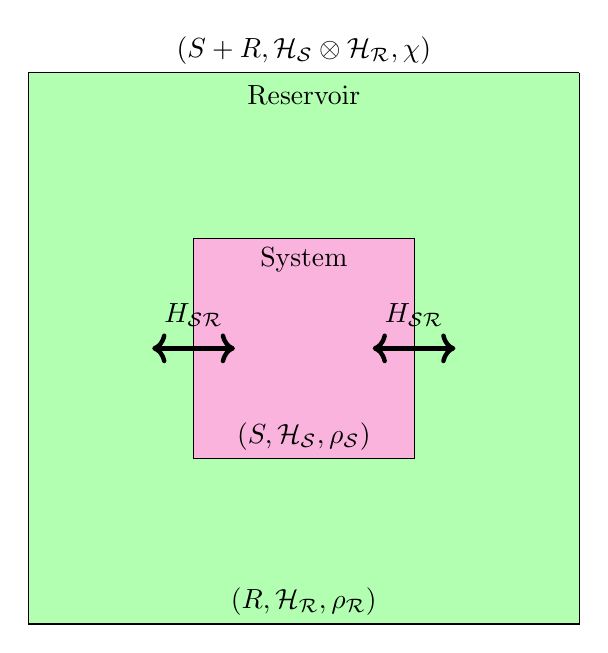
\begin{tikzpicture}[scale=.7]
\draw [fill=green!30] (10,10) -- (0,10) -- (0,0) -- (10,0)--(10,10);
\node at (5,10.4) {\scalebox{1.0}{$\left(S+R, \mathcal{H}_{\mathcal{S}} \otimes \mathcal{H}_{\mathcal{R}}, \chi \right)$}} ;
\draw [fill=magenta!30] (7,7) rectangle (3,3 );
\node at (5,.4) { \scalebox{1.0}{\textcolor{black}{$\left(R, \mathcal{H}_{\mathcal{R}}, \rho_{\mathcal{R}} \right)$}} };
\node at (5,3.4) {\scalebox{1.0}{$\left(S, \mathcal{H}_{\mathcal{S}}, \rho_{\mathcal{S}} \right)$}};
\draw[ultra thick, <->] (2.25,5) -- (3.75,5);
\draw[ultra thick, <->] (6.25,5) -- (7.75,5);
\node at (3,5.6) {\scalebox{1.0}{$H_{\mathcal{SR}}$}};
\node at (7,5.6) {\scalebox{1.0}{$H_{\mathcal{SR}}$}};
\node at (5,6.6) {\scalebox{1.0}{System}};
\node at (5,9.6) {\scalebox{1.0}{Reservoir}};
\end{tikzpicture}
\caption{Partitioning of the full Hilbert space into system and reservoir subspaces.}
\label{Hilbert_Space}
\end{figure}
%
To zoom in on the slow dynamics caused by the interaction $H_{\mathcal{SR}}$, we move into the interaction picture. Defining 
\begin{equation}\label{full_dentity_matrix_interaction_picture}
\tilde{\chi}(t) = e^{i (H_{\mathcal{S}} + H_{\mathcal{R}})t/\hbar} \chi e^{- i (H_{\mathcal{S}} + H_{\mathcal{R}})t/\hbar}
\end{equation}
and taking the time derivative of Eq. (\ref{full_dentity_matrix_interaction_picture}), we obtain
\begin{eqnarray}\label{density_matrix_dynamics_interaction_picture}
\dot{\tilde{\chi} } & = & \frac{i}{\hbar} (H_{\mathcal{R}} + H_{\mathcal{S}} )\tilde{\chi} - \frac{i}{\hbar}\tilde{\chi} (H_{\mathcal{R}} + H_{\mathcal{S}} )+ e^{i (H_{\mathcal{S}} + H_{\mathcal{R}})t/\hbar} \dot{\chi} e^{- i (H_{\mathcal{S}} + H_{\mathcal{R}})t/\hbar} \nonumber \\
& =&  - \frac{i}{\hbar} [\tilde{H}_{\mathcal{SR}}(t) , \tilde{\chi}(t)],
\end{eqnarray}
where
\begin{equation}
\tilde{H}_{\mathcal{SR}}(t) = e^{i (H_{\mathcal{S}}+H_{\mathcal{R}})t/\hbar} H_{\mathcal{SR}} e^{-i (H_{\mathcal{S}}+H_{\mathcal{R}})t/\hbar}.
\end{equation}
The formal solution to this equation is
\begin{equation}\label{Formal_Soltuion_Density_Matrix_Interaction_Picture}
\tilde{\chi}(t) = \chi(0) - \frac{i}{\hbar} \int_0^t ds \, [\tilde{H}_{\mathcal{SR}}(s) , \tilde{\chi}(s)].
\end{equation}
Note that $\tilde{\chi}(0) = \chi(0)$. Substituting the formal solution, Eq. (\ref{Formal_Soltuion_Density_Matrix_Interaction_Picture}), in Eq. (\ref{density_matrix_dynamics_interaction_picture}), we obtain the equation for the full density operator in the interaction picture
\begin{equation}
\dot{\tilde{\chi}}  =  -\frac{i}{\hbar} [ \tilde{H}_{\mathcal{SR}}(t), \chi(0) ] - \frac{1}{\hbar^2} \int_0^t ds \, [\tilde{H}_{\mathcal{SR}}(t), [\tilde{H}_{\mathcal{SR}}(s), \tilde{\chi}(s)]].
\end{equation}
In order to obtain an equation describing dynamics of the reduced system, $S$, we partial trace over the reservoir degrees of freedom
\begin{equation}\label{Exact_density_matrix_dynamics}
\dot{\tilde{\rho}} =  - \frac{1}{\hbar^2} \int_0^t ds \,  tr_{\mathcal{R}} \left\lbrace [\tilde{H}_{\mathcal{SR}}(t), [\tilde{H}_{\mathcal{SR}}(s), \tilde{\chi}(s)]] \right\rbrace.
\end{equation}
Here, $\tilde{\rho}_{\mathcal{S}}(t) = tr_{\mathcal{R}}\left\lbrace \tilde{\chi} (t)\right\rbrace$ and we assumed that
\begin{equation}\label{Traceless_assumption}
tr_{\mathcal{R}}  \left\lbrace [ \tilde{H}_{\mathcal{SR}} (t), \chi(0) ] \right\rbrace = 0.
\end{equation} 
The assumption is true when the reservoir is in the vacuum state; for any general state of the reservoir this can be ensured by adding the term $tr_{\mathcal{R}} \left\lbrace H_{\mathcal{SR}} \rho_{\mathcal{R}} \right\rbrace$ to the system Hamiltonian \cite{StatMethQOI}. At this stage Eq. (\ref{Exact_density_matrix_dynamics}) is exact since no approximations have been made so far.
%However, the dynamics of the density matrix have been cast into a form where reasonable approximations can be made.
%
%ccccccccccccccccccccccccccccccccccccccccc
\subsection{Born-Markov Approximation}
%cccccccccccccccccccccccccccccccccccccccc
%
The first assumption that is made is the system and reservoir begin uncorrelated and remain uncorrelated because $H_{\mathcal{SR}}$ is weak. Furthermore, it is assumed that density operator of the environment is time-independent. This implies,
%
\begin{equation}
\tilde{\chi}(t) = \tilde{\rho}_{\mathcal{S}}(t) \otimes \rho_{\mathcal{R}}. 
\end{equation}
so
\begin{equation}\label{non_markovian_master_equation}
\dot{\tilde{\rho}}_{\mathcal{S}} =  - \frac{1}{\hbar^2} \int_0^t ds \,  tr_{\mathcal{R}} \left\lbrace [\tilde{H}_I(t), [\tilde{H}_I(s), \tilde{\rho}_{\mathcal{S}}(s) \otimes \rho_{\mathcal{R}}]] \right\rbrace.
\end{equation}
Typically correlations (entanglement) between the subsystems build up because of the interaction. Thus we are assuming the reservoir is so large, compared to the system, that it is virtually unaffected by the coupling to the system. This equation is sometimes called the Redfield equation which was developed in the context of nuclear magnetic resonance \cite{IBM}. %For concerns we will considered exclusively reservoir in the thermal state


%At this point   Eq. ()Next $\tilde{\rho}_S(s) \rightarrow \tilde{\rho}_S(t)$ which says that th. This equation is called the Redfield equation, which isn't yet Markovian because it doesn't have so we make a substation, $s=t-\tau$ and extend the limits of integration to infinity.
%\begin{equation}
%\dot{\tilde{\rho}} = - \frac{1}{\hbar^2} \int_0^\infty d\tau \, \,  tr_R \left\lbrace [\tilde{H}_I(t), [\tilde{H}_I(t - \tau), \rho_S(t) \otimes \rho_R.]] \right\rbrace
%\end{equation}

To proceed any further, we have to be more specific about the form of the interaction. Since the interaction acts on both subspaces, without loss of generality, we can decompose the interaction as 
%
\begin{equation}\label{Tensor_Product_Interaction}
H_{\mathcal{SR}} = \hbar  \sum_\alpha A_\alpha \otimes b_\alpha^\dagger + h.c. 
\end{equation}
%
where $b_\alpha^\dagger$ denotes the creation operator for a given oscillator comprising the reservoir. Then moving into the interaction picture, this gives
\begin{equation}
\tilde{H}_{\mathcal{SR}}(t)  =  \hbar  \sum_\alpha A_\alpha(t) \otimes b_\alpha^\dagger(t) + h.c.
\end{equation}
where $A_\alpha(t)= e^{i H_{\mathcal{S}} t / \hbar } A_\alpha e^{- i H_{\mathcal{S}} t /\hbar }$ and $b_\alpha(t) = e^{i H_{\mathcal{R}} t/ \hbar } b_\alpha e^{-i H_{\mathcal{R}} t /\hbar }$. For a reservoir in a thermal state at temperature $T$, the density operator can be written as,
%
\begin{equation}
\rho_{\mathcal{R}} = \frac{1}{tr_{\mathcal{R}} \lbrace e^{-H_{\mathcal{R}} / k T} \rbrace} e^{-H_{\mathcal{R}} / k T}.
\end{equation}
%
where $H_{\mathcal{R}} = \hbar \sum_\alpha \omega_\alpha b_\alpha^\dagger b_\alpha$. We are now able to trace over the reservoir degrees of freedom
%
\begin{align}
\dot{\tilde{\rho}}_{\mathcal{S}} & =  \sum_{\alpha \beta } \int_{0}^{t} d\tau \;  \biggl\lbrace \left[   A_\beta (t-\tau) \tilde{\rho}_{\mathcal{S}} , A_\alpha(t) \right] \left\langle b_\alpha(t) b_\beta(t-\tau) \right\rangle \nonumber \\
& \quad + \left[   A_\beta^\dagger (t-\tau) \tilde{\rho}_{\mathcal{S}} , A_\alpha^\dagger(t) \right] \left\langle b_\alpha^\dagger(t) b_\beta^\dagger (t-\tau) \right\rangle  \nonumber \\
& \quad + \left[  A_{\beta}^\dagger(t-\tau) \tilde{\rho}_{\mathcal{S}} , A_\alpha(t)   \right] \left\langle b_\alpha(t) b_\beta^\dagger(t-\tau)  \right\rangle \nonumber \\
& \quad + \left[  A_{\beta}(t-\tau) \tilde{\rho}_{\mathcal{S}} , A_\alpha^\dagger(t)   \right] \left\langle b_\alpha^\dagger(t) b_\beta(t-\tau)  \right\rangle + h.c. \biggr\rbrace 
\label{Eq:rho1}
\end{align} 
%
To proceed any further we need to evaluate the correlation functions of the reservoir. For a Markovian reservoir, these correlation functions decay more rapidly than any timescale associated with the system. Ideally, they would decay instantaneously i.e. \cite{StatMethQOI}
%
\begin{equation}
\left\langle b_\alpha^{\dagger}(t) b_\beta(s) \right\rangle \sim \delta(t-s).
\end{equation}
%
Calculating the correlation functions explicitly, we find
\begin{eqnarray}
\left\langle b_\alpha(t) b_\beta(t-\tau) \right\rangle & = & \left\langle b_\alpha^\dagger(t) b_\beta^\dagger(t-\tau) \right\rangle = 0 \\
\left\langle b_\alpha^\dagger(t) b_\beta(t-\tau) \right\rangle & = & \gamma_\alpha N( \omega_\alpha ) \delta_{\alpha \beta} \delta(\tau) \\
\left\langle b_\alpha(t) b_\beta^\dagger(t-\tau) \right\rangle & = & \gamma_\alpha (1+N( \omega_\alpha )) \delta_{\alpha \beta} \delta(\tau) 
\end{eqnarray}
where 
\begin{equation}
N_\omega_{\alpha} = \frac{1}{e^{\hbar\omega_{\alpha}/k_B T} - 1}
\end{equation}
is the Bose-Einstein occupation number. Substituting the correlation functions in Eq. (\ref{Eq:rho1}), we obtain
\begin{align}
\dot{\tilde{\rho}}_{\mathcal{S}} & =  \sum_{\alpha } \gamma_\alpha \left\lbrace \left[  A_{\alpha}^\dagger(t) \tilde{\rho}_{\mathcal{S}} , A_\alpha(t)   \right] \left( 1 + N(\omega_\alpha) \right) + \left[  A_{\alpha}(t) \tilde{\rho}_{\mathcal{S}} , A_\alpha^\dagger(t)   \right] N( \omega_\alpha ) + h.c. \right\rbrace \nonumber
\end{align} 
Moving back into the Schrodinger picture using
\begin{equation}
 \dot{\rho}_{\mathcal{S}} = -\frac{i}{\hbar} [H_{\mathcal{S}}, \rho_{\mathcal{S}} ] + e^{-i H_{\mathcal{S}} t} \left( \frac{d}{d t } \dot{\tilde{\rho}}_{\mathcal{S}} \right) e^{ i H_{\mathcal{S}} t }
\end{equation}
we find
\begin{align}
\dot{\rho}_{\mathcal{S}} & = -\frac{i}{\hbar}[H_{\mathcal{S}}, \rho_{\mathcal{S}}] + \sum_{\alpha} \gamma_\alpha \left\lbrace \left[  A_{\alpha}^\dagger \rho_{\mathcal{S}} , A_\alpha   \right] \left( 1 + N(\omega_\alpha) \right) + \left[  A_{\alpha} \rho_{\mathcal{S}} , A_\alpha^\dagger   \right] N( \omega_\alpha ) + h.c. \right\rbrace . \nonumber
\end{align} 
Expanding out the commutators we can write 
\begin{align}\label{Effective_dynamics}
\dot{\rho}_{\mathcal{S}} & = - \frac{i}{\hbar} [H_{\mathcal{S}}, \rho_{\mathcal{S}} ] \\
& \quad +  \sum_{\alpha } \frac{\gamma_\alpha}{2} \biggl[ (1 + N_{\omega_\alpha} ) \left( A_\alpha \rho_{\mathcal{S}} A_\alpha^\dagger + \frac{1}{2} \left\lbrace A_\alpha^\dagger A_\alpha , \rho_{\mathcal{S}} \right\rbrace \right) \nonumber\\
& \quad +  N_{\omega_\alpha}  \left( A_\alpha^\dagger \rho_{\mathcal{S}} A_\alpha +\frac{1}{2} \left\lbrace A_\alpha A_\alpha^\dagger , \rho_{\mathcal{S}} \right\rbrace \right)\biggr]. \nonumber
\end{align} 
We now have have an equation that captures the effective dynamics of the open system $\mathcal{S}$. Typically, $A_\alpha$ is proportional to a lowering operator. This makes the second term describe decay of the system into the reservoir, with a rate proportional $\gamma_\alpha(1+N_{\omega_k})$.  And the third term proportional to absorption of the system from the reservoir.
%
%cccccccccccccccccccccccccccccccccccccccccccccccccc
\section{Optical Bloch Equations}
%cccccccccccccccccccccccccccccccccccccccccccccccccccc
%
We now present a simple example of a driven-dissipative two-level system (a.k.a. qubit), coupled to a reservoir, with an XX-type interaction. The total Hamiltonian is is the sum $H=H_{\mathcal{S}} + H_{\mathcal{R}} + H_{\mathcal{SR}}$, where
%
\begin{eqnarray}
H_{\mathcal{R}} & = & \omega_c b^\dagger b \nonumber \\
H_{\mathcal{S}} & = & \frac{\epsilon}{2} \sigma_z + \Omega \cos( \omega_l t )\sigma_x \nonumber \\
H_{\mathcal{SR}} & = & g \sigma_{x} \sum_{\alpha} \left( b_{\alpha} + b_{\alpha}^\dagger \right).
\end{eqnarray}
%
To avoid the fast dynamics caused by the drive we move into a rotating frame (RF) with a unitary 
\begin{equation}
    U = exp\left(-i \left\{\sum_{\alpha} \omega_\alpha b_{\alpha}^\dagger b_{\alpha} + \frac{\omega_l}{2} \sigma_z\right\}\right)
\end{equation} 
%
This transforms $b_{\alpha} \rightarrow b_{\alpha}e^{-i \omega_{\alpha} t} $ and $\sigma \rightarrow \sigma e^{- i \omega_l t }$ thus modifying the different pieces of the Hamiltonian as (see Appendix A),
%
\begin{eqnarray}
& & H_{\mathcal{R}}' = 0 \nonumber \\
& & H_{\mathcal{S}}' \approx \frac{\delta}{2} \sigma_z + \frac{\Omega}{2}(e^{i\omega_l t}+e^{-i\omega_l t})(\sigma e^{-i\omega_l t} + \sigma^{\dagger}e^{i\omega_l t})\nonumber \\
& & H_{\mathcal{SR}}' =  g\sum_{\alpha} ( b_{\alpha} e^{- i \omega_{\alpha} t}+ b^\dagger e^{ i \omega_{\alpha} t} ) ( \sigma e^{ - i \omega_l t } + \sigma^\dagger e^{ i \omega_l t }),
\end{eqnarray}
%
where we have expressed cosine function in terms of exponential. The symbol ${\delta = \epsilon - \omega_l}$ denotes the detuning of qubit resonant frequency and the drive frequency system. Ignoring fast oscillating terms under a rotating wave approximation (RWA)\cite{RWA}, the resultant Hamiltonian is
%
\begin{eqnarray}\label{Jaynes_Cummings_Optical_Block}
& & H_{\mathcal{S}}' \approx \frac{\delta}{2} \sigma_z + \frac{\Omega}{2}\sigma_{x} \nonumber\\
& & H_{\mathcal{SR}}' \approx g \sum_\alpha (\sigma b_{\alpha}^\dagger e^{-i \Delta t} + h.c.),
\end{eqnarray} 
%
where $\Delta = \omega_{l} -\omega_{\alpha}$. The interaction in Eq. (\ref{Jaynes_Cummings_Optical_Block}) is often called the Jaynes-Cummings interaction. Comparing it to Eq.(\ref{Tensor_Product_Interaction}) and identifying $A_\alpha = \sigma$. Substituting into Eq. (\ref{Effective_dynamics}), we can write the master equation for this driven-dissipative qubit as
%
\begin{align}\label{Optical Block ME}
\dot{\rho}_{\mathcal{S}} & =  - i \frac{\delta}{2} [ \sigma_z, \rho ] - i \frac{\Omega}{2} [ \sigma_x , \rho ] \nonumber \\
& \quad + \gamma ( 1 + N_{\omega_b} ) \left( \sigma \rho_{\mathcal{S}} \sigma^\dagger - \frac{1}{2} \left\lbrace \sigma^\dagger \sigma , \rho_{\mathcal{S}} \right\rbrace \right) + \gamma N_{\omega_b} \left( \sigma^\dagger \rho_{\mathcal{S}} \sigma - \frac{1}{2} \left\lbrace \sigma \sigma^\dagger , \rho_{\mathcal{S}} \right\rbrace \right),
\end{align}
%
with $N_{\omega_b} = Tr\{\rho_{B}b^{\dagger}b\}$. In writing this equation, we have assumed $(\omega_{\alpha} - \omega_{l}) \ll \tau_{\mathcal{R}}^{-1}$, where $\tau_{\mathcal{R}}$ is the relaxation time of the reservoir \cite{TheoryOfOpen}. The second term in this equation is responsible for decay into the reservoir, at a rate $\gamma ( 1 + N_{\omega_b} )$. This rate captures both simulated emission that scales with bath occupation number (i.e. $\gamma N_{\omega_b}$) and spontaneous emission $\gamma$ corresponding to decay induced due to vacuum fluctuations. The third term is responsible for absorption into the system at a rate $\gamma N_{\omega_b}$.  
%
\begin{figure}[t!]
\centering
\includegraphics[width=0.9\textwidth]{decoherence}
\caption{(Left Panel) Numerical simulation of optical Bloch equations showing a decay of Rabi oscillations. (Right panel) Furthermore, the expectation values of all the Pauli operators are  decaying towards zero which means that the steady state of qubit is a mixed state. Since excitations leave and enter the system stochastically (i.e. not coherently) its not surprising the state has decohered \cite{WF_approach_Quantum_Dyanmics}.}
\label{Fig:OBESim}
\end{figure}
%
\par
%
The expectation values for the Pauli operators are
\begin{eqnarray}
\left\langle \dot{\sigma}_x \right\rangle & = & - \gamma \left( 2 N_{\omega_b} + 1 \right) \left\langle \sigma_x \right\rangle - \delta \left\langle \sigma_y \right\rangle \nonumber \\
\left\langle \dot{\sigma}_y \right\rangle & = & \delta \left\langle \sigma_{x} \right\rangle - \gamma \left( 2 N_{\omega_b} + 1 \right) - \Omega \left\langle \sigma_z \right\rangle \nonumber \\
\left\langle \dot{\sigma}_z \right\rangle & = & \Omega \left\langle \sigma_y \right\rangle - 2 \gamma [ \left\langle \sigma_z \right\rangle ( 2 N_{\omega_{b}} + 1 ) + 1  ].
\end{eqnarray}
%
They are called optical Bloch equations. Numerical simulations in Fig. \ref{Fig:OBESim} show that the expectation values of Pauli operators decay to zero. 
%
\par
%
The steady state density matrix of Eq. (\ref{Optical Block ME}) was found to be
\begin{equation}\label{Eqn:Decohered_Steady_State}
\rho_S \xrightarrow{t\rightarrow\infty} \frac{1}{2} \left( | e \rangle \langle e | + | g \rangle \langle g | \right),
\end{equation}
which is referred to as a mixed state, and is distinguished from 
a coherent superposition,
\begin{equation}\label{Eqn:Coherent_Superposition}
|\Psi\rangle_{S} = \frac{1}{\sqrt{2}}\left( |e \rangle + e^{i\phi} | g \rangle \right),
\end{equation}
which we called a pure state. Though the probabilities of being found in the excited or ground state are same for both the pure and mixed state, their origins are quite different. The probabilities associated with Eq. (\ref{Eqn:Decohered_Steady_State}) arise from the uncertainty in the state of the system. This is in contrast with Eq. (\ref{Eqn:Coherent_Superposition}) where the state can be represented with a well-defined ket in $\mathcal{H}_{S}$. The probabilities of $1/2$ obtained from measurement of such a superposition are intrinsic to quantum mechanics, and not necessarily due to ignorance or uncertainty about the state of the system as is the case for a statistical mixture. 

Another way to see this is that there is a fixed phase relationship between the states $|e\rangle$ and $|g\rangle$ in Eq. (\ref{Eqn:Coherent_Superposition}) that contains vital information about its orientation on the Bloch sphere. There is no phase relation between the excited and ground state in Eq. (\ref{Eqn:Decohered_Steady_State}) however. This evolution of a state into a statistical mixture, resulting in the loss of encoded coherent information, is referred to as decoherence.
%We expand the density matrix as $\rho = \mathcal{I} + \vec{\sigma} \cdot \vec{r}$ where $\vec{r} = \langle \vec{\sigma} \rangle$. 
%Because $\rho \xrightarrow{\vec{r}\rightarrow 0} \mathcal{I}$ the steady state is mixed \cite{NAZIRNOTES}.
%
%Let us review what we just did did, find the effective dynamics of $S$ we will use the intereaction piture to zoom in the "slow" dynamics created by the weak interaction between the $S$ and $R$. We assume that $S+R$ forms a closed system, and apply unitary evolution to the system. Then making the Bohn-Markov approximation we partial trace over the environmental degrees of freedom to get an effective description of the dyanamics of the reduced system. We will see that this effective description can be put into "Lindbald form," and the this equaiton often leads to dechoherence. We will then consider under what conditions is this Lindbald master equation able to stabilized pure states.






%\section{Adiabatic Elimination and Engineered Dissipation }

%Typically w there are excited states that have population in them for short period of time. Typically we are concern with $n$ two-level systems interacting with a lossy oci


%\textcolor{blue}{This derivation need to connect the Charmicheal antz $\chi = \rho_S |0 \rangle_R \langle 0 |$ to $\langle \dot{a} \rangle \approx 0 $}
%
%|
%
%\textcolor{blue}{What is the reason for going into the rotating frame and then ignoring the time dependence of the operators?}
%
%| 
% 
%\textcolor{blue}{Also thinking about making a diagram for section or when I }
%
%|
%
%\textcolor{blue}{I am going to have to think of a way to simplify/summarize this derivation.}
%
%||||||||




% Chapter 2: Two Spin Bell State Stabilization
%---------------------------------------------------------------------
\chapter{Bell State Stabilization}
%ccccccccccccccccccccccccccccccccccccccccccc
%
As evident from the results presented in last chapter, dissipation destroys quantum coherences leading to steady states that are statistical mixtures of classical states. In this chapter, we will show how dissipation seen by the quantum systems can be engineered such that the system settles into a pure quantum state. Specifically, since Bell states are important to quantum information platforms, we will present a protocol where the steady state of dissipation-driven two-qubit system is
%
\begin{equation}
\rho \xrightarrow{t\rightarrow\infty} \left|\Phi\right\rangle\left\langle\Phi \right|,
\end{equation}
%
where $\left|\Phi \right\rangle = (\left|eg \right\rangle- \left|ge \right\rangle)/\sqrt{2}$ is a maximally entangled singlet state. 
%
\par
%
We will first introduce the Liouvillian superoperator that describes the evolution of an open quantum system (analogous to the Hamiltonian describing the evolution of a closed quantum system). This description will allow us to introduce the notions of fidelity and gap for a stabilization protocol. We will then describe the conditions that need to be satisfied for a dissipative process to have a pure steady state --- in particular, we detail the method of adiabatic elimination that allows to eliminate bath modes constituting a fast subspace of the problem and write engineered dissipators seen by the reduced quantum system of interest. We will then use this method to analyze a system of two qubits coupled to a lossy resonator. We will consider two specific cases:
%
\begin{itemize}
\item \emph{Symmetric Case}: In this case the two qubits effectively ``talk" to each other through the resonator mode, which manifests itself as an effective dissipative interaction between the qubits once the resonator mode is eliminated. 
\item \emph{Chiral Case}: In this we will add a direct coherent interaction between the qubits, and tune the relative phase between the dissipative and coherent interactions such that one qubit ``sees" the other but not vice-versa. 
\end{itemize}
%
%
%ccccccccccccccccccccccccccccccccccccccccccccccccccccccccccc
\section{Liouvillian}
%ccccccccccccccccccccccccccccccccccccccccccccccccccccccccccc
%
In essence, the quantum master (GKSL) equation introduced in the previous chapter is the Liouville-von Neumann equation plus a dissipator, defined as
%
\begin{equation}
\mathcal{D}[c_l] \rho = \left( c_l \rho c_l^\dagger - \frac{1}{2} \left\lbrace c_l^\dagger c_l , \rho \right\rbrace \right)
\end{equation}
%
The dissipator is a function of a quantum jump operator, $c_l$, that captures the ``engineered" decay/absorption process with an associated rate $\gamma_l \geq 0$. Whether the dissipator is associated with decay/absorption into the reservoir depends if the collapse operator is proportional to a creation or annihilation operator. Here we rewrite the quantum master equation as an eigenvalue equation 
%
\begin{eqnarray}
\dot{\rho} = \mathcal{L}\rho
\end{eqnarray}
%
by defining the Liouvillian superoperator as

\begin{equation}
\mathcal{L}\bullet = - \frac{i}{\hbar} [ H , \bullet ] + \sum_n \gamma_l \left( c_l \bullet c_l^\dagger - \frac{1}{2} \left\lbrace c_l^\dagger c_l , \bullet \right\rbrace \right).
\end{equation}
%
Using the above notation, we can write the formal solution to GKSL equation as
%
\begin{equation}\label{Eqn:Formal Dynamical map}
\rho(t) = e^{\mathcal{L}t } \rho(0).
\end{equation}
%
Note that this assumes that the Hamiltonian and jump operators are time-independent.
%
\par
%
Converting the Liouvillian superoperator, $\mathcal{L} \bullet$, converted into an $n^2 \times n^2 $ matrix, $L$, and the density matrix, $\rho$, into a $n^2 \times 1$ column vector we write the formal solution \ref{Eqn:Formal Dynamical map} in terms of the eigenvalues of $L$.
\begin{equation}
\vec{\rho}(t) = e^{\mathcal{L}t} \vec{\rho} =  \sum_n e^{\lambda_n} \vec{\rho}_n
\end{equation}
For simplicity we are assuming non-degeneracy. It turns out the Liouvillian matrix has a single zero eigenvalue with the rest coming in conjugate pairs with a negative real part. The eigenvector corresponding to zero is the steady state, $\rho_{ss}$, because $\rho \xrightarrow{t\rightarrow\infty} \rho_{ss}$. The speed at which a system approaches $\rho_{ss}$ is called the gap, $\Delta_\mathcal{L}$, and is equal to the eigenvalue with the smallest real part \cite{KrausTheorems}. How ``close" the steady state is to a bell state, $| \Phi \rangle$. The metric of this ``closeness" is called the fidelity and is defined as 
\begin{equation}
F_{| \Phi \rangle} = tr \lbrace | \Phi \rangle \langle \Phi |  \rho_{ss} \rbrace.
\end{equation}

%
%ccccccccccccccccccccccccccccccccccccccccccccccccccc
\section{Dark States}
%ccccccccccccccccccccccccccccccccccccccccccccccccccc
%
We rewrite the Liouvillian in terms of the positive map, $\mathcal{E}(\rho) = 2 \sum_l \gamma_l c_l \rho c_l^\dagger$, and $Q = P - i H$, with $P = \sum_ l \gamma_l c_l^\dagger c_l$ \cite{KrausTheorems}.
\begin{equation}\label{Liovillian Alternative}
\mathcal{L}\rho = \mathcal{E}(\rho) - Q^\dagger \rho - \rho Q 
\end{equation}
%A steady state is time independent and th
\begin{thm}\label{Theorem}
Let $\mathcal{L}$ be defined as in Eq. (\ref{Liovillian Alternative}). Then $\mathcal{L}\left( |\Phi \rangle \langle \Phi |  \right)=0$ if and only if the following two conditions are satisfied: 

(1) $Q^\dagger | \Phi \rangle = \lambda | \Phi \rangle$ for some $\lambda \in \mathbb{C}$

(2) $c_l | \Phi \rangle = \lambda_l | \Phi \rangle$ for some $\lambda_l \in \mathbb{C}$ with $\sum_l g_l |\lambda_l|^ 2 = Re ( \lambda ) $.

\end{thm}

\begin{proof}
If $\mathcal{L}( \left| \Phi \> \< \Phi \right|  ) = 0$ then 

\begin{eqnarray}\label{Kraus SigmaX}
\mathcal{E} \left( \left| \Phi \> \< \Phi \right| \right) & = & Q^\dagger \left| \Phi \> \< \Phi \right| + \left| \Phi \> \< \Phi \right| Q  \nonumber \\
2 \sum_l g_l \left| \Psi_l \> \< \Psi_l \right| & = & \left| \Phi \> \< \eta \right| + \left| \eta \> \< \Phi \right|  
\end{eqnarray}
with $\left| \Psi_l \right\rangle = c_l \left| \Phi \right\rangle$ and $Q^\dagger \left| \Phi \right\rangle = \left| \chi \right\rangle$. Since the left-hand-side of Eq. (\ref{Kraus SigmaX}) is a positive operator (ie. $g_l \geq 0$), the right-hand-side must also be a positive operator. However, the right-hand-side is a Pauli $\sigma_x$ operator in bra-ket notation which has a negative eigenvalue, a contradiction. It can be shown that $A=\left| \Phi \> \< \eta \right| + \left| \eta \> \< \Phi \right|$ is positive if and only if its rank is one, that is $\left| \chi \right\rangle = \lambda \left| \Phi \right\rangle$ for some $\lambda \in \mathbb{C}$
\begin{equation}
Q^\dagger \left| \Phi \right\rangle = \left| \chi \right\rangle = \lambda \left| \Phi \right\rangle.
\end{equation}
Thus condition $\textit{(1)}$ is satisfied. Rewriting Eq. (\ref{Kraus SigmaX})
\begin{equation}
2 \sum_l g_l \left| \Psi_l \> \< \Psi_l \right| = 2 \Re(\lambda) \left| \Phi \> \< \Phi \right|
\end{equation}
note that both sides are positive. The above equation must be satisfied for all $\left| \Phi \right\rangle$. This can only be true when $c_l \left| \Phi \right\rangle= \lambda_l \left| \Phi \right\rangle$ and $\sum_l g_l |\lambda_l|^2 =\Re(\lambda) $.
\end{proof}
%
\par
%
We define a \textbf{dark state} as a state that is an eigenstate of a Hamiltonian ($H^{(D)}$) and set of jump operators $(c_l^{(D)})$. Rearranging conditions $(1)$ and $(2)$
\begin{eqnarray}\label{Eqn:DarkStateConditions}
H^{(D)} | \Phi \rangle & = & \Im{\lambda} | \Phi \rangle \nonumber \\ 
c_l^{(D)} | \Phi \rangle & = & 0
\end{eqnarray}
the steady state, $| \Phi \rangle$, is an eigenstate of the Hamiltonian $H^{(D)} = H - i \sum_l g_l \lambda_l (c_l')^\dagger + i \sum g_l \lambda_l^* c_l$, and a null ket of the jump operator $c_l^{(D)} = c_l - \lambda_l$.
Physically these conditions mean, in addition to being a stationary state of the unitary dynamics, a dark state cannot absorb or emit a photon.  

%The full system, considered in section 2.4, has a lossy resonator mode that facilitates the stabilization of a bell state. However, the resonator decay route does not say anything about the dark space of the qubits. Thus the quasi-static resonator mode is adiabatically eliminated.
%\subsection{Dark States}
%
%The engineered quantum jump operator that we are interested in is proportional to an angular momentum lowering operator, that is $\hat{S} = \sigma_1 + \sigma_2 + \sigma_3 + ...$, which only has zero eigenvalues (ie. $\lambda_l = 0$). This implies that $\lambda = 0$, and that conditions $\textit{(1)}$ and $\textit{(2)}$ of Theorem \ref{Theorem} become
%\begin{eqnarray}
%\hat{S} \left| \Psi \> = 0 \nonumber \\
%H \left| \Psi \> = 0.
%\end{eqnarray}
%Therefore, to stabilize a bell state the null space of the engineered jump operator is determined. The space spanned by the null space will be called dark states, labeled $\left| D \>$. Then insisting that the dark state satisfy $ H \left| D \> =0$ what parameter have to be chosen such that $\left| D \> \longrightarrow \left| S \>$ can be determined.
%
%ccccccccccccccccccccccccccccccccccccccccccccccccccccccccccc
\section{Adiabatic Elimination of Reservoir}
%cccccccccccccccccccccccccccccccccccccccccccccccccccccccccc
%
We consider a general adiabatic elimination of a low/medium Q-value resonator mode, coupled to an arbitrary system $\mathcal{S}$ with a weak Jaynes-Cummings interaction. Due to the low Q-value of the resonator, we assume weak coupling i.e. $\kappa \gg g$. In this regime, the following ansatz is valid 
%
\begin{equation}\label{ansatz}
\chi \approx \rho_S(t) \otimes \left| 0 \>_R \< 0 \right|.
\end{equation}
%
We consider the Hamiltonian
\begin{equation}
H=H_S + H_R + H_{SR}
\end{equation}
where
\begin{eqnarray}\label{D_AB}
\frac{H_R}{\hbar} & = & \Delta b^{\dagger} b \nonumber \\
\frac{H_{SR}}{\hbar} & = & g \left( b^{\dagger} \hat{S} e^{i \phi } + b \hat{S}^{\dagger} e^{-i \phi} \right). 
\end{eqnarray}
and $\hat{S}$ is an arbitrary system operator ($\hat{S} \in \mathcal{H}_S$). The quantum master (GKSL) equation, expressed in superoperator notation, with resonator decay is
\begin{eqnarray}\label{Schrodinger Superoperator}
\frac{d}{dt}\chi & = & \left( \mathcal{L}_R + \mathcal{L}_S + \mathcal{L}_{SR} \right) \chi
\nonumber \\
\mathcal{L}_R \bullet &=& - \frac{i}{\hbar} [ H_R , \bullet ] + \kappa \mathcal{D}[b]\bullet \nonumber \\
\mathcal{L}_S \bullet  &=& - \frac{i}{\hbar} [ H_S, \bullet ]  \nonumber \\
\mathcal{L}_{SR} \bullet & = & - \frac{i}{\hbar} [H_{SR} , \bullet ].
\end{eqnarray}
Moving into the interaction picture, we can write
\begin{eqnarray}\label{Eqn:Super_Interaction_Pic}
\tilde{\chi} &= &e^{-( \mathcal{L}_S + \mathcal{L}_R ) t } \chi \nonumber \\
\frac{d}{dt} \tilde{\chi} & = & \mathcal{\tilde{L}}_{SR}(t) \tilde{\chi} \nonumber \\
\mathcal{\tilde{L}}_{SR}(t) &= & e^{-( \mathcal{L}_S + \mathcal{L}_R ) t } \mathcal{L}_{SR} e^{( \mathcal{L}_S + \mathcal{L}_R ) t }.
\end{eqnarray}
%Our goal is to find $\tilde{\mathcal{L}}_{SR}(t)$. 
Using the factorization property of superoperators, namely $AB\bullet = (A \bullet ) ( B \bullet )$ and $\bullet A B = ( \bullet A ) ( \bullet B )$, $\mathcal{\tilde{L}}_{RS}(t)$ can be factorized into time-dependent system and reservoir superoperators.
\begin{eqnarray}
\mathcal{\tilde{L}}_{SR}(t) & = & -ig \lbrace \mathcal{R}_2'(t) \mathcal{S}_1'(t) e^{ i \phi } + \mathcal{R}_1'(t) \mathcal{S}_2'(t) e^{- i \phi} - \mathcal{R}_2'^{\dagger} (t) \mathcal{S}_1'^{\dagger}(t) e^{- i \phi} - \mathcal{R}_1'^{\dagger}(t) \mathcal{S}_2^{\dagger}(t) e^{i \phi }  \rbrace \nonumber \\
 & = & - i g \left[ (b^{\dagger} \bullet )' ( \hat{S} \bullet ) ' e^{i \phi } - ( \bullet b^{\dagger} )' ( \bullet \hat{S} )' e^{ i \phi } + ( b \bullet )' ( \hat{S}^{\dagger} \bullet )' e^{ - i \phi } - (\bullet b)' (\bullet \hat{S}^{\dagger} )' e^{- i \phi } \right] \nonumber \\
\mathcal{S}_1'(t) & = & ( \hat{S} \bullet)'= e^{-  \mathcal{L}_S t } \hat{S} \bullet e^{  \mathcal{L}_S t } \nonumber \\
\mathcal{R}_1'(t) & = & (b \bullet)' = e^{- \mathcal{L}_R t } b \bullet e^{\mathcal{L}_R t} \nonumber \\
\mathcal{S}_2'(t) & = & (\hat{S}^{\dagger} \bullet)' =  e^{- \mathcal{L}_S t } \hat{S}^{\dagger} \bullet e^{ \mathcal{L}_S t } \nonumber \\
\mathcal{R}_2'(t) &=& (b^{\dagger} \bullet )' = e^{-\mathcal{L}_R t } b^{\dagger} \bullet e^{\mathcal{L}_R t } \nonumber 
\end{eqnarray}

 Time dependent superoperators of the form $\mathcal{O}(t) = e^{- \mathcal{L} t } S e^{\mathcal{L} t }$ satisfy Heisenberg-like equation
\begin{equation}
\frac{d }{d t} \mathcal{O}(t) = [ \mathcal{O} , \mathcal{L} ].
\end{equation}
Sparing the reader, we relegate the mathematical details to Appendix B, and directly present the final solutions to the operators below:
\begin{eqnarray}
\mathcal{R}_1'(t) &=& \left( b \bullet \right)' =  \left( b \bullet \right) e^{- \left( i \Delta + \frac{\kappa }{2} \right) t } \nonumber \\
\mathcal{R}_1'^{\dagger} (t) & = & \left( \bullet b^{\dagger} \right)' = \left( \bullet b^{\dagger} \right) e^{\left( i \Delta - \frac{\kappa}{2} \right) t} \nonumber \\
\mathcal{R}_2'(t) & = & \left( b^{\dagger} \bullet \right)' = \left( b^{\dagger} \bullet \right) e^{(i \Delta + \frac{\kappa}{2})t} - \left( \bullet b^{\dagger} \right) e^{i \Delta t}\left( e^{\kappa t / 2} - e^{- \kappa t / 2 } \right) \nonumber \\
\mathcal{R}_2'^{\dagger}(t) & = & \left( \bullet b \right)' = \left( \bullet b \right) e^{ \left( - i \Delta + \frac{\kappa}{2} \right) t} - \left( b \bullet \right) \left( e^{\kappa t / 2} - e^{- \kappa t / 2 } \right).
\end{eqnarray}
As a check, note that $\left( b \bullet \right)' = ( b \bullet )$ and $\left( b^\dagger \bullet \right)' = ( b^\dagger \bullet )$ at $t=0$.
%
\par%
Substituting the above solutions in Eq. (\ref{Eqn:Super_Interaction_Pic}) and tracing over the reservoir to capture the effective dynamics of the reduced system, we obtain 
\begin{equation}
\frac{d}{d t} \tilde{\rho}_S =   \int_0^t d\tau \; tr_R \left\lbrace \mathcal{\tilde{L}}_{SR}(t) \mathcal{\tilde{L}}_{SR}(\tau) \tilde{\rho}_S(t) \left| 0 \>_R \< 0 \right| \right\rbrace.
\end{equation}
Note that $tr_R \left\lbrace \mathcal{\tilde{L}}_{SR}(t) \tilde{\rho}_S(t) \left| 0 \>_R \< 0 \right| \right\rbrace=0$
because $\langle 0 | b | 0 \rangle = \langle 0 | b^{\dagger} | 0 \rangle = 0$.
We find that second-order product is decaying as the time difference $t-\tau$ increases. This is the reservoir correlation function.
\begin{align}\label{decay expodential}
tr_R \lbrace \mathcal{\tilde{L}}_{SR}(t) \mathcal{\tilde{L}}_{SR}(\tau) \tilde{\chi} \rbrace & =  g^2 e^{ - \kappa ( t - \tau )/ 2 } \lbrace \mathcal{S}_1'^{\dagger}(t) \mathcal{S}_1'(\tau) \nonumber \\
& \quad +  \mathcal{S}_1'(t) \mathcal{S}_1'^{\dagger}(\tau) - \mathcal{S}_2'^{\dagger}(t) \mathcal{S}_1'^{\dagger}(\tau) - \mathcal{S}_2'(t) \mathcal{S}_1'(t) \rbrace \tilde{\rho}_S(t) \nonumber \\
\end{align}
In the Markovian limit, the correlation function decays instantaneously i.e. $e^{ - \kappa ( t - \tau ) / 2} \rightarrow  2 \delta( t - \tau ) / \kappa$. This leads us to the following equation \cite{StatMethQOI,StatMethQOII} for the system density operator,
\begin{equation}
\frac{d}{dt } \tilde{\rho}_S = \frac{2 g^2}{\kappa} \lbrace 2 \mathcal{S}_1'^{\dagger}(t) \mathcal{S}_1(t) - \mathcal{S}_2'^{\dagger}(t) \mathcal{S}_1'^{\dagger}(t) - \mathcal{S}_2'(t) \mathcal{S}_1'(t) \rbrace \tilde{\rho}_S(t)
\end{equation}
Substituting the definitions of $\mathcal{S}_1'(t)$ and $\mathcal{S}_2'(t)$,
remembering $\rho_S = e^{\mathcal{L}_S t }\tilde{\rho}_S$, taking a derivative, simplifying, rearranging, and using $\mathcal{L}_S\rho_S = - \frac{i}{\hbar} [ H_S, \rho_S ]$ we arrive at
\begin{eqnarray} \label{Engineered Reduced System}
\frac{d}{d t} \rho_S & = & - \frac{i}{\hbar} [ H_S, \rho_S ] + \frac{2 g^2}{\kappa} \left\lbrace 2 \hat{S} \rho_S \hat{S}^{\dagger} - \hat{S}^{\dagger} \hat{S} \rho_S - \rho_S \hat{S}^{\dagger} \hat{S} \right\rbrace \nonumber \\
& = & - \frac{i}{\hbar} [H_S, \rho_S] + \frac{4 g^2}{\kappa} \mathcal{D}[\hat{S}] \rho_S.
\end{eqnarray}
The reduced system undergoes unitary evolution in conjunction with dissipative process given by the ``engineered" jump operator $\hat{S}$. Furthermore, adiabatic elimination allows us to read off the ``engineered" dissipation rate seen by the system as $\Gamma = \frac{4 g^2}{\kappa}$. Our next task is to find the operator $\hat{S}$ that makes a two-qubit system decay into a Bell state.
%
%cccccccccccccccccccccccccccccccc
\section{Bell State Stabilization}
%cccccccccccccccccccccccccccccccc
%
\subsection{Symmetric Scheme}
We will consider two driven qubits interacting with a single resonator mode, as depicted in Fig. \ref{LevelDiagram}(a). This is a standard situation encountered in platforms such as circuit-QED \cite{Wallraff2004}. The lab frame Hamiltonian describing the system is,
\begin{equation}\label{Two Quipt Pamametric Couplings}
\frac{H}{\hbar} = \omega_c b^\dagger b + \sum_{i=1}^2 \left\{ \frac{\omega_i}{2}\sigma_{zi} + \Omega_i \cos \left( \omega_{li} t \right) \sigma_{xi} + g_i \sigma_{xi} \left( b + b^\dagger \right)\right\}.
\end{equation}
We avoid the fast dynamics caused by the drives by changing into a rotating frame with the  unitary
%
\begin{equation}\label{Equ:Rotating_Hamiltonian}
U = \exp\left(-i\left\{\omega_c b^\dagger b + \sum_{i=1}^{2} \frac{\omega_{li}}{2}\sigma_{zi}\right\}\right).
\end{equation}
%
Transforming the Hamiltonian in this frame as $H' = \mathcal{U} H \mathcal{U}^\dagger - H_{rot}$ (see Appendix A) and performing RWA, we find
%
\begin{eqnarray}\label{Two_Qubit_Hamiltonian}
\frac{H'_R}{\hbar} & = & 0 \nonumber \\
\frac{H'_S}{\hbar} & \approx & \sum_{i=1}^2 \left( \frac{\delta_i}{2}  \sigma_{zi}  + \frac{\Omega_i}{2} \sigma_{xi} \right) \nonumber \\
\frac{H'_{SR}}{\hbar} & \approx &  b^\dagger \underbrace{( g_1 \sigma_1 + g_2 \sigma_2 )}_\text{$=g\hat{S}$} + h.c. 
\end{eqnarray} 
%
with detunings $ \delta_i = \omega_i -\omega_{li}$. Note that we have assumed resonance between the cavity and qubit driving field, i.e., $\omega_c = \omega_{l1} = \omega_{l2}$. Comparing the interaction Hamiltonian with Eq. (\ref{D_AB}) we conclude that the effective jump operator is $g\hat{S} = g_1 \sigma_1 + g_2 \sigma_2$ giving the engineered dissipator,
%
\begin{eqnarray}
\mathcal{D}[\hat{S}] = \mathcal{D}[g_1 \sigma_1 + g_2 \sigma_2].
\end{eqnarray}
%
Writing the resultant master equation describing the two-qubit open system, we obtain
%
\begin{align}\label{Expand reduced system ME}
\dot{\rho}_S  & = - \frac{i}{\hbar} [H'_S, \rho_S] + \frac{4 g_1^2}{\kappa}\mathcal{D}[\sigma_1]\rho_S +  \frac{4 g_2^2}{\kappa}\mathcal{D}[\sigma_2]\rho_S \nonumber \\
& \quad + \frac{4  g_1 g_2 }{\kappa} \bigg[  \left(\sigma_1 \rho_S \sigma_2^\dagger - \frac{1}{2} \left \lbrace \sigma_2^\dagger \sigma_1 , \rho_S \right\rbrace \right) + \left( \sigma_2 \rho_S \sigma_1^\dagger - \frac{1}{2} \left \lbrace \sigma_1^\dagger \sigma_2 , \rho_S \right\rbrace \right) \biggr].
\end{align}
%
where we have factored the engineered dissiparor into single-qubit and two-qubit dissipation terms explicitly. Expressed in this form each qubit experiences relaxation at rate proportional to $4 g_i^2 / \kappa$. The final terms in Eq. (\ref{Expand reduced system ME}) give rise to a dissipative interaction (between the qubits Alice and Bob) with a strength proportional to $4 g_1 g_2 / \kappa$ [Fig. \ref{LevelDiagram}(b)].

For the purposes of bell-state stabilization the couplings and drives need to be homogeneous. That is $g_1 = g_2 = g$, and $\Omega_1 = \Omega_2 = \Omega$. Under these conditions the jump operator $\hat{S}$ has zero eigenvalues exclusively, $\lambda_l=0$ in Eq. (\ref{Eqn:DarkStateConditions}), and its null space spans contains dark states of the form
%
\begin{equation}
\label{Two qubit Dark State}
|\Phi\rangle =\frac{1}{\sqrt{1 + |\alpha|^2 }} \left(| g g\rangle + \alpha | S\rangle \right)
\end{equation}
%
where $\alpha$ is called the singlet fraction. Furthermore, condition \textit{(2)} of \textbf{Theorem \ref{Theorem}} becomes $H_S'|\Phi\rangle=0$. This constraint on the parameters requires 
%
\begin{equation}
\delta = \delta_1 = - \delta_2; \quad {\rm and} \quad \alpha = \frac{\Omega}{\sqrt{2} \delta}.
\end{equation}
%
When the qubit drives are strong and resonant,  $|\Phi \rangle \xrightarrow{\alpha\rightarrow\infty}| S \rangle$, a high-fidelity singlet state is stabilized. This was verified numerically in Fig. \ref{LevelDiagram}(d).
%
%\begin{equation}
%H \left| D \> = -\frac{1}{2} \left( \delta_1 + \delta_2 \right)\left| gg \> + \left[ \frac{\alpha}{\sqrt{2}} \left( \frac{\delta_2}{2} - \frac{\delta_1}{2} \right) + \frac{\Omega}{2} \right] \left| g e \> + \left[ \frac{\alpha}{\sqrt{2}} \left( \frac{\delta_2}{2} - \frac{\delta_1}{2} \right) + \frac{\Omega}{2} \right] \left| e g \> \nonumber
%\end{equation}
%
%
\subsection{Chiral Scheme}
%
We again consider the system of two qubits coupled to common resonator, but with an additional time-dependent coupling between the qubits, Fig. \ref{ChiralLevelDiagram}(a). The Hamiltonian for this system is
%
\begin{equation}
\frac{H}{\hbar} = \omega_c b^\dagger b + \sum_{i=1}^2 \left\{ \frac{\omega_i}{2}\sigma_{zi} + \Omega_i \cos \left( \omega_{li} t \right) \sigma_{xi}+ g_i \sigma_{xi} (b + b^\dagger)\right\} + M_{12}(t) \sigma_{x1} \sigma_{x2}
\end{equation}
%
where $M_{12}(t) = J e^{i \omega_p t} + c.c$. As before, we isolate the slow dynamics of the interaction by moving into a rotating frame with the unitary given in Eq. (\ref{Equ:Rotating_Hamiltonian}). Picking the modulation frequency to be the difference, $\omega_p = \omega_{l1} - \omega_{l2}$. Post RWA, the Hamiltonian is
 \begin{eqnarray}\label{Two_Qubit_Hamiltonian}
\frac{H'_R}{\hbar} & = & 0 \nonumber \\
\frac{H'_S}{\hbar} & = & \sum_{i=1}^2 \left( \frac{\delta_i}{2}  \sigma_{zi}  + \frac{\Omega_i}{2} \sigma_{x1} \right) + J \sigma_1 \sigma_2^\dagger + J^* \sigma_1^\dagger \sigma_2 \nonumber \\
\frac{H'_{SR}}{\hbar} & = &  b^\dagger ( g_1 \sigma_1 + g_2 \sigma_2 ) + h.c. 
\end{eqnarray} 
%where there are additional qubit-qubit coupling terms added to the system Hamiltonian. %The master equation for the reduced full system are still given by Eq. (\ref{reduced system ME}) and Eq. (\ref{Master Equation Full}), respectfully.

%Let us now add on some additios qubit-qubit coupling term (shown in red) to the system Hamilton in Eq. (\ref{Two_Qubit_Hamiltonian}) so that it is know of the form
%\begin{equation}\label{qubit-qubit coupling hamiltonian}
%\frac{H_S}{\hbar} = \frac{\delta_1}{2}  \sigma_{z1} + \frac{\delta_2}{2} \sigma_{z2} + \Omega ( \sigma_{x1} + \sigma_{x2} ) + \textcolor{red}{J \sigma_1 \sigma_2^\dagger + J^* \sigma_1^\dagger \sigma_2}. 
%\end{equation}
The master equation for the reduced system is same as Eq. (\ref{Expand reduced system ME}), since the qubit-resonator coupling remains unchanged, except with an additional coupling term in $H'_S$. Using it, we calculate expectation values of single qubit operators and find % along with  defined as $\langle \dot{A} \rangle = tr_s \left\lbrace A \dot{\rho}_S \right\rbrace$), can the cyclic property of traces (ie. $tr\left( A B \right) = tr \left( B A \right)$). Through which we find
\begin{eqnarray}
\frac{d}{d t} \langle \sigma_1 \rangle & = &  - i \Delta_1 \langle \sigma_1 \rangle + i \Omega_1 \langle \sigma_{z1} \rangle + \left( iJ^* + \frac{\Gamma}{2} \right) \langle \sigma_{z1} \sigma_2 \rangle - \frac{\Gamma}{2} \langle \sigma_1 \rangle  \nonumber \\
\frac{d}{dt } \langle \sigma_2 \rangle &=& - i \Delta_2 \langle \sigma_2 \rangle + i \Omega_2 \langle \sigma_{z2} \rangle + \left( i J + \frac{\Gamma}{2} \right) \langle \sigma_1 \sigma_{z2} \rangle  - \frac{\Gamma}{2} \langle \sigma_2 \rangle \nonumber 
\end{eqnarray}
If the strength and phase of the qubit-qubit couplings are tuned such that
\begin{equation}\label{Chirality_Condition}
\boxed{ J = \pm i \frac{\Gamma}{2} }
\end{equation} 
then one qubit sees the other but not vice versa. The boxed equation is called the chirality condition, which has previously been employed to implement nonreciprocal amplification and frequency conversion \cite{PhysRevLett.113.247003,PhysRevX.5.021025,PhysRevApplied.7.034031}. Assuming 
homogeneous drives and couplings, the dark state is the same as the symmetric case, Eq. (\ref{Two qubit Dark State}). The constraint $H_S' | \Phi \rangle  = 0 $ implies $\delta_1 = - \delta_2 = \delta$ and \cite{Chiral_QO_of_Spin_Chains,Chiral_QO_of_V_Level}
\begin{equation}
    \alpha = \frac{\sqrt{2}\Omega}{2 \delta + i \Gamma}.
\end{equation}
Results of numerical simulations in Fig. \ref{ChiralLevelDiagram}(d) show that the chiral scheme stabilizes a high-fidelity singlet-state when $\alpha \rightarrow \infty$.
%
\begin{figure}[h!]
\subfigure[]{
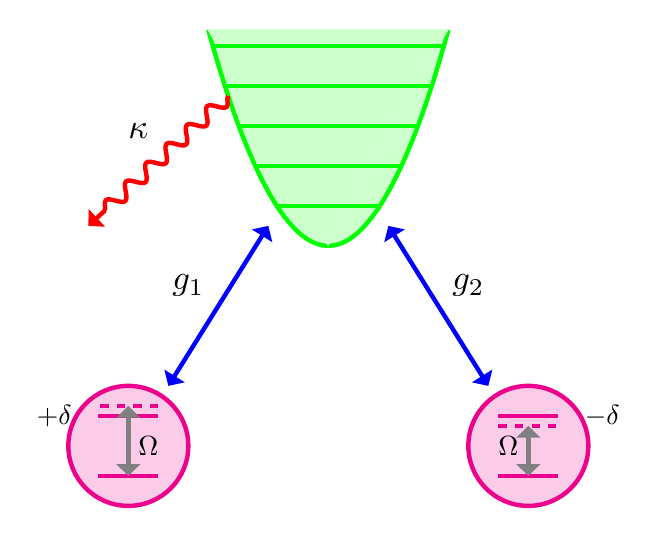
\begin{tikzpicture}[x=1.0in,y=1.0in]
\filldraw[color=green!100, fill=green!20 , ultra thick] (0,0) parabola (0.6,1.08) ;
\filldraw[color=green!100, fill=green!20 , ultra thick] (0.0,0.0) parabola (-0.6,1.08) ;
\filldraw[color= magenta!100, fill=magenta!20, ultra thick](-1,-1) circle (.3);
\filldraw[color=magenta!100, fill=magenta!20, ultra thick](1,-1) circle (.3);
\filldraw[color=green!20, fill=green!20] (0,0) -- ( -0.6,1.08) -- ( 0.6,1.08);
\draw[blue, ultra thick , tipA-tipA] (-0.8,-.7) -- (-0.3,0.1);
\draw[blue, ultra thick , tipA-tipA] (0.8,-.7) -- (0.3,0.1);
\draw [red, ultra thick,-tipA,decorate,decoration={snake,post length=1.65mm}] (-.5,.75) -- (-1.2, .1);
\node at (-.95,.575) {\scalebox{1.25}{$\kappa$}} ;
\draw[color= magenta!100 , ultra thick] (-.85,-1.15)--(-1.15,-1.15);
\draw[color= magenta!100 , ultra thick] (-.85,-.85)--(-1.15,-0.85);
\draw[color= magenta!100 , ultra thick] (.85,-1.15)--(1.15,-1.15);
\draw[color= magenta!100 , ultra thick] (.85,-.85)--(1.15,-0.85);
\draw [dashed,color= magenta!100 , ultra thick] (.85,-.90)--(1.15,-0.90);
\draw [dashed,color= magenta!100 , ultra thick] (-.85,-.80)--(-1.15,-0.80);
\draw [gray, ultra thick , tipA-tipA] (-1.0,-1.15)--(-1.0,-.8);
\draw [gray, ultra thick , tipA-tipA] (1.0,-1.15)--(1.0,-.9);
\node at (-0.9,-1.0) {\scalebox{1.0}{$\Omega$}} ;
\node at (0.9,-1.0) {\scalebox{1.0}{$\Omega$}} ;
\node at (-1.37,-0.85) {\scalebox{1.0}{$+\delta$}} ;
\node at (1.37,-0.85) {\scalebox{1.0}{$-\delta$}} ;
\draw[color=green!100 , ultra thick] (-0.36514837167011072,.4) -- (0.36514837167011072,.4);
\draw[color=green!100 , ultra thick] (0.2581988897471611,.2) -- (-0.2581988897471611,.2);
\draw[color=green!100 , ultra thick] (0.44721359549995793,.6) -- (-0.44721359549995793,.6);
\draw[color=green!100 , ultra thick] (0.5163977794943222,.8) -- (-0.5163977794943222,.8);
\draw[color=green!100 , ultra thick] (0.57735026918962573,1.0) -- (-0.57735026918962573,1.0);
\node at (.7, -.2) {\scalebox{1.25}{$g_2$}} ;
\node at (-.7, -.2) {\scalebox{1.25}{$g_1$}} ;
\end{tikzpicture}
}
\hspace*{-.3cm}
\subfigure[]{
\raisebox{-2cm}{
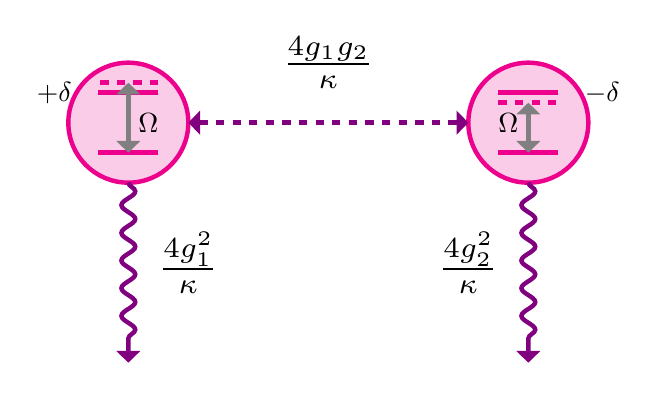
\begin{tikzpicture}[x=1.0in,y=1.0in]
\filldraw[color= magenta!100, fill=magenta!20, ultra thick](-.6,-1) circle (.3);
\filldraw[color=magenta!100, fill=magenta!20, ultra thick](1.4,-1) circle (.3);
\draw[color= magenta!100 , ultra thick] (-.45,-1.15)--(-0.75,-1.15);
\draw[color= magenta!100 , ultra thick] (-.45,-.85)--(-0.75,-0.85);
\draw[color= magenta!100 , ultra thick] (1.25,-1.15)--(1.55,-1.15);
\draw[color= magenta!100 , ultra thick] (1.25,-.85)--(1.55,-0.85);
\draw[violet , ultra thick , dashed , tipA-tipA] (-.3, -1.0) --(1.1,-1.0);
%\draw[orange , ultra thick , dashed , tipA-] (-.3, -1.15) --(1.1,-1.15);
\draw[violet , ultra thick , -tipA , decorate , decoration={snake,post length=1.65mm}] (-.6, -1.3) --(-.6,-2.2);
\draw[violet , ultra thick , -tipA , decorate , decoration={snake,post length=1.65mm}] (1.4, -1.3) --(1.4,-2.2);
\node at (-0.5,-1.0) {\scalebox{1.0}{$\Omega$}} ;
\node at (1.3,-1.0) {\scalebox{1.0}{$\Omega$}} ;
\node at (-0.97,-0.85) {\scalebox{1.0}{$+\delta$}} ;
\node at (1.77,-0.85) {\scalebox{1.0}{$-\delta$}} ;
\draw [gray, ultra thick , tipA-tipA] (-0.6,-1.15)--(-0.6,-.8);
\draw [gray, ultra thick , tipA-tipA] (1.4,-1.15)--(1.4,-.9);
\draw [dashed,color= magenta!100 , ultra thick] (1.25,-.90)--(1.55,-0.90);
\draw [dashed,color= magenta!100 , ultra thick] (-.45,-.80)--(-0.75,-0.80);
\node at (0.4,-.7) {\scalebox{1.5}{$\frac{4 g_1  g_2 }{\kappa}$}} ;
\node at (-0.3,-1.7) {\scalebox{1.5}{$\frac{4 g_1^2}{\kappa}$}} ;
\node at (1.1,-1.7) {\scalebox{1.5}{$\frac{4 g_2^2}{\kappa}$}} ;
\end{tikzpicture}
}
}

\subfigure[]{
%\raisebox
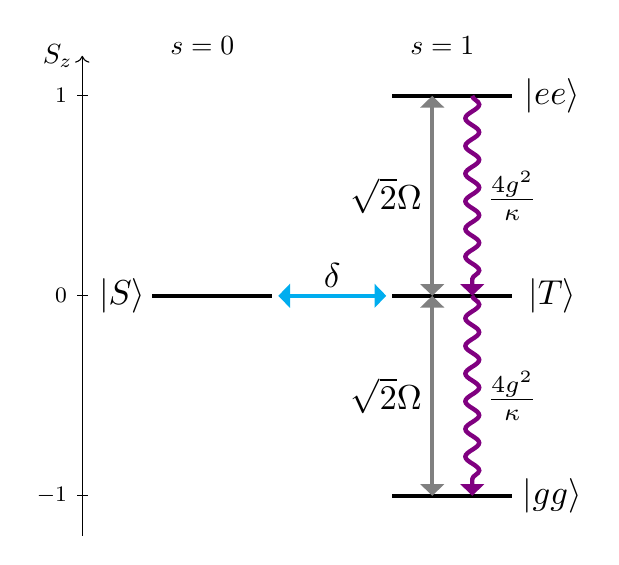
\begin{tikzpicture}[x=1.0in,y=1.0in]
%\begin{scope}[shift={(-1.0in,0.0in)}]
\draw[ultra thick] (0.3,0.0) -- (0.90,0.0);
\draw[ultra thick] (1.5,-1.0) -- (2.1,-1.0);
\draw[ultra thick] (1.5,0.0) -- (2.1,0.0);
\draw[ultra thick] (1.5,1.0) -- (2.1,1.0);
\node at (0.15,0.0) {\scalebox{1.25}{$\left| S \right\rangle$}} ;
\node at (2.30,-1.0) {\scalebox{1.25}{$\left| gg \right\rangle$}} ;
\node at (2.30,0.0) {\scalebox{1.25}{$\left| T \right\rangle$}} ;
\node at (2.30,1.0) {\scalebox{1.25}{$\left| ee \right\rangle$}} ;
\node at (1.47,-.5) {\scalebox{1.25}{$\sqrt{2} \Omega$}} ;
\node at (1.47,0.5) {\scalebox{1.25}{$\sqrt{2} \Omega$}} ;
\node at (2.1,-.5) {\scalebox{1.25}{$\frac{4g^2}{\kappa}$}} ;
\node at (2.1,.5) {\scalebox{1.25}{$\frac{4g^2}{\kappa}$}} ;
%\node at (6.0,3.0) {\scalebox{1.0}{$\frac{8g^2}{\kappa}$}} ;
%\node at (6.0,1.0) {\scalebox{1.0}{$\frac{8g^2}{\kappa}$}} ;
\draw[cyan, ultra thick , tipA-tipA] (.93,0) -- (1.47,0);
\node at (1.2, 0.1) {\scalebox{1.25}{$ \delta $}};
\draw[gray, ultra thick , tipA-tipA] (1.7,-1) -- (1.7,0);
\draw[gray, ultra thick , tipA-tipA] (1.7,0) -- (1.7,1);
%\draw[gray, ultra thick , tipA-tipA] (4.6,2) -- (4.6,4);
%%\draw[red, ultra thick, tipA-,decorate, decoration={ snake , post length=2mm }  ] (5.4,0) -- (5.4,2);
%%\draw[red, ultra thick, tipA-,decorate, decoration={snake}] (5.4,2) -- (5.4,4);
%\draw [red, ultra thick,-tipA,decorate,decoration={snake,post length=1.65mm}] (5.4,4) -- (5.4,2);
\draw [violet, ultra thick,-tipA,decorate,decoration={snake,post length=1.65mm}] (1.9,0) -- (1.9,-1);
\draw [violet, ultra thick,-tipA,decorate,decoration={snake,post length=1.65mm}] (1.9,1) -- (1.9,0);
\node at (0.55,1.25) {\scalebox{1.0}{$s=0$}} ;
\node at (1.75,1.25) {\scalebox{1.0}{$s=1$}} ;
\draw[->,yshift=1.0in] (-0.05,-2.2) -- (-.05,0.2) node[left] {$S_z$};
\foreach \y in {-1,0,1} \draw[shift={(-0.05,\y)}] (2pt,0pt) --(-2pt,0pt) node[left] {\footnotesize $\y$};
%\end{scope}
\end{tikzpicture}
}
\hspace*{-.25in}
\subfigure[]{
\includegraphics[width=3.5in,height=2.75in]{Sym_stabilization.pdf}
}

\caption{(a) Graphical depiction of two qubits coupled to a lossy resonator mode. (b) After the resonator mode is adiabatically eliminated the resonator decay (red) and the resonator-qubit interactions (blue) merge to create an engineered dissipator (purple). This ``engineered" dissipator gives rise to local qubit relaxation and a dissipative interaction between qubits. (c) Graphical depiction of how the states couple for homogeneous drives and couplings. (d) Master equation simulations of both the full and reduced systems, show high-fidelity stabilization of a singlet state for strong resonant drives.}
\label{LevelDiagram}
\end{figure}
%
\begin{figure} 
\subfigure[]{
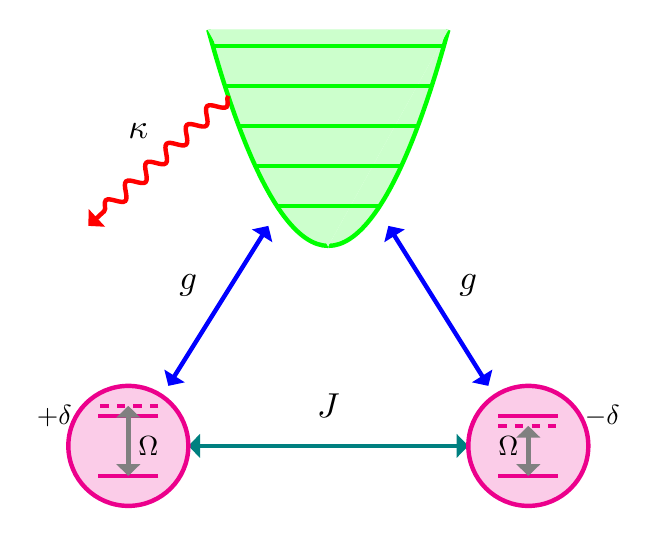
\begin{tikzpicture}[x=1.0in,y=1.0in]
\filldraw[color=green!100, fill=green!20 , ultra thick] (0,0) parabola (0.6,1.08) ;
\filldraw[color=green!100, fill=green!20 , ultra thick] (0.0,0.0) parabola (-0.6,1.08) ;
\draw[teal , ultra thick , tipA-tipA] (-.7, -1) -- (.7, -1) ;
\node at (0, -0.8) {\scalebox{1.25}{$J$}} ;
\filldraw[color= magenta!100, fill=magenta!20, ultra thick](-1,-1) circle (.3);
\filldraw[color=magenta!100, fill=magenta!20, ultra thick](1,-1) circle (.3);
\filldraw[color=green!20, fill=green!20] (0,0) -- ( -0.6,1.08) -- ( 0.6,1.08);
\draw[blue, ultra thick , tipA-tipA] (-0.8,-.7) -- (-0.3,0.1);
\draw[blue, ultra thick , tipA-tipA] (0.8,-.7) -- (0.3,0.1);
\node at (.7, -.2) {\scalebox{1.25}{$g$}} ;
\node at (-.7, -.2) {\scalebox{1.25}{$g$}} ;
\node at (-.95,.575) {\scalebox{1.25}{$\kappa$}} ;
\draw [red, ultra thick,-tipA,decorate,decoration={snake,post length=1.65mm}] (-.5,.75) -- (-1.2, .1);
\draw[color= magenta!100 , ultra thick] (-.85,-1.15)--(-1.15,-1.15);
\draw[color= magenta!100 , ultra thick] (-.85,-.85)--(-1.15,-0.85);
\draw[color= magenta!100 , ultra thick] (.85,-1.15)--(1.15,-1.15);
\draw[color= magenta!100 , ultra thick] (.85,-.85)--(1.15,-0.85);
\draw [dashed,color= magenta!100 , ultra thick] (.85,-.90)--(1.15,-0.90);
\draw [dashed,color= magenta!100 , ultra thick] (-.85,-.80)--(-1.15,-0.80);
\draw [gray, ultra thick , tipA-tipA] (-1.0,-1.15)--(-1.0,-.8);
\draw [gray, ultra thick , tipA-tipA] (1.0,-1.15)--(1.0,-.9);
\node at (-0.9,-1.0) {\scalebox{1.0}{$\Omega$}} ;
\node at (0.9,-1.0) {\scalebox{1.0}{$\Omega$}} ;
\node at (-1.37,-0.85) {\scalebox{1.0}{$+\delta$}} ;
\node at (1.37,-0.85) {\scalebox{1.0}{$-\delta$}} ;
\draw[color=green!100 , ultra thick] (-0.36514837167011072,.4) -- (0.36514837167011072,.4);
\draw[color=green!100 , ultra thick] (0.2581988897471611,.2) -- (-0.2581988897471611,.2);
\draw[color=green!100 , ultra thick] (0.44721359549995793,.6) -- (-0.44721359549995793,.6);
\draw[color=green!100 , ultra thick] (0.5163977794943222,.8) -- (-0.5163977794943222,.8);
\draw[color=green!100 , ultra thick] (0.57735026918962573,1.0) -- (-0.57735026918962573,1.0);
\end{tikzpicture}
}
\hspace*{-.3in}
\subfigure[]{
\raisebox{-2cm}{
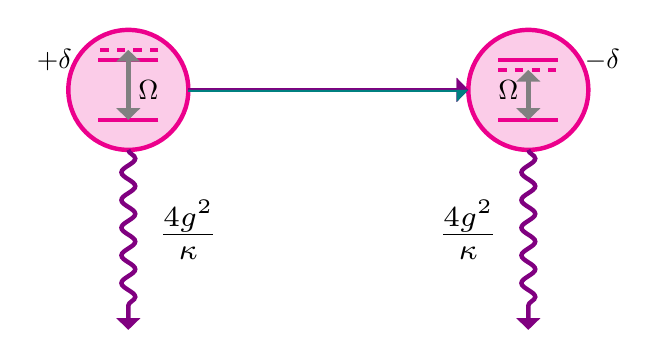
\begin{tikzpicture}[x=1.0in,y=1.0in]
\filldraw[color= magenta!100, fill=magenta!20, ultra thick](-.6,-1) circle (.3);
\filldraw[color=magenta!100, fill=magenta!20, ultra thick](1.4,-1) circle (.3);
\draw[color= magenta!100 , ultra thick] (-.45,-1.15)--(-0.75,-1.15);
\draw[color= magenta!100 , ultra thick] (-.45,-.85)--(-0.75,-0.85);
\draw[color= magenta!100 , ultra thick] (1.25,-1.15)--(1.55,-1.15);
\draw[color= magenta!100 , ultra thick] (1.25,-.85)--(1.55,-0.85);
\draw[ violet , ultra thick  , -tipA] (-.3, -1.0) --(1.1,-1.0);
%\draw[orange , ultra thick , dashed , tipA-] (-.3, -1.15) --(1.1,-1.15);
\draw[violet , ultra thick , -tipA , decorate , decoration={snake,post length=1.65mm}] (-.6, -1.3) --(-.6,-2.2);
\draw[violet , ultra thick , -tipA , decorate , decoration={snake,post length=1.65mm}] (1.4, -1.3) --(1.4,-2.2);
   \def\mypath{ (-.3, -1.0) --(1.1,-1.0)}
    \draw[color=violet ,  ultra thick , -tipA] \mypath;
    \begin{scope}[overlay]
      \clip (-1, -1) -- \mypath -- ++(1, 0) -- ++(0, -2) -- cycle;
      \draw[color=teal, -tipA , ultra thick] \mypath;
    \end{scope}
\node at (-0.5,-1.0) {\scalebox{1.0}{$\Omega$}} ;
\node at (1.3,-1.0) {\scalebox{1.0}{$\Omega$}} ;
\node at (-0.97,-0.85) {\scalebox{1.0}{$+\delta$}} ;
\node at (1.77,-0.85) {\scalebox{1.0}{$-\delta$}} ;
\draw [gray, ultra thick , tipA-tipA] (-0.6,-1.15)--(-0.6,-.8);
\draw [gray, ultra thick , tipA-tipA] (1.4,-1.15)--(1.4,-.9);
\draw [dashed,color= magenta!100 , ultra thick] (1.25,-.90)--(1.55,-0.90);
\draw [dashed,color= magenta!100 , ultra thick] (-.45,-.80)--(-0.75,-0.80);
%\node at (0.4,-.7) {\scalebox{1.5}{$\frac{8\left| g_1 \right| \left| g_2 \right|}{\kappa}$}} ;
\node at (-0.3,-1.7) {\scalebox{1.5}{$\frac{4 g^2}{\kappa}$}} ;
\node at (1.1,-1.7) {\scalebox{1.5}{$\frac{4 g^2}{\kappa}$}} ;
\end{tikzpicture}
}
}

\subfigure[]{
%\raisebox
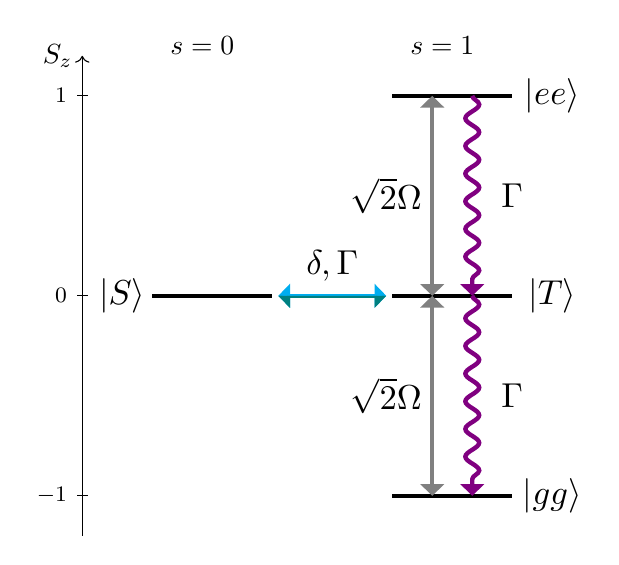
\begin{tikzpicture}[x=1.0in,y=1.0in]
\draw[ultra thick] (0.3,0.0) -- (0.90,0.0);
\draw[ultra thick] (1.5,-1.0) -- (2.1,-1.0);
\draw[ultra thick] (1.5,0.0) -- (2.1,0.0);
\draw[ultra thick] (1.5,1.0) -- (2.1,1.0);
\node at (0.15,0.0) {\scalebox{1.25}{$\left| S \right\rangle$}} ;
\node at (2.30,-1.0) {\scalebox{1.25}{$\left| gg \right\rangle$}} ;
\node at (2.30,0.0) {\scalebox{1.25}{$\left| T \right\rangle$}} ;
\node at (2.30,1.0) {\scalebox{1.25}{$\left| ee \right\rangle$}} ;
\node at (1.47,.5) {\scalebox{1.25}{$\sqrt{2} \Omega$}} ;
\node at (1.47,-.5) {\scalebox{1.25}{$\sqrt{2} \Omega$}} ;
\node at (2.1,-.5) {\scalebox{1.25}{$\Gamma$}} ;
\node at (2.1,.5) {\scalebox{1.25}{$\Gamma$}} ;
%\node at (6.0,3.0) {\scalebox{1.0}{$\frac{8g^2}{\kappa}$}} ;
%\node at (6.0,1.0) {\scalebox{1.0}{$\frac{8g^2}{\kappa}$}} ;
    \def\mypath{(.93,0) -- (1.47,0)}
    \draw[color=cyan , ultra thick , tipA-tipA] \mypath;
    \begin{scope}[overlay]
      \clip (-1, -1) -- \mypath -- ++(1, 0) -- ++(0, -2) -- cycle;
      \draw[color=teal, tipA-tipA , ultra thick] \mypath;
    \end{scope}
%\draw[cyan, ultra thick , tipA-tipA] (.93,1) -- (1.47,1);
\node at (1.2, 0.15) {\scalebox{1.25}{$ \delta , \Gamma$}};
\draw[gray, ultra thick , tipA-tipA] (1.7,-1) -- (1.7,0);
\draw[gray, ultra thick , tipA-tipA] (1.7,0) -- (1.7,1);
%\draw[gray, ultra thick , tipA-tipA] (4.6,2) -- (4.6,4);
%%\draw[red, ultra thick, tipA-,decorate, decoration={ snake , post length=2mm }  ] (5.4,0) -- (5.4,2);
%%\draw[red, ultra thick, tipA-,decorate, decoration={snake}] (5.4,2) -- (5.4,4);
%\draw [red, ultra thick,-tipA,decorate,decoration={snake,post length=1.65mm}] (5.4,4) -- (5.4,2);
\draw [violet, ultra thick,-tipA,decorate,decoration={snake,post length=1.65mm}] (1.9,0) -- (1.9,-1);
\draw [violet, ultra thick,-tipA,decorate,decoration={snake,post length=1.65mm}] (1.9,1) -- (1.9,0);
\node at (0.55,1.25) {\scalebox{1.0}{$s=0$}} ;
\node at (1.75,1.25) {\scalebox{1.0}{$s=1$}} ;
\draw[->] (-0.05,-1.2) -- (-.05,1.2) node[left] {$S_z$};
\foreach \y in {-1,0,1} \draw[shift={(-0.05,\y)}] (2pt,0pt) --(-2pt,0pt) node[left] {\footnotesize $\y$};
\end{tikzpicture}
}
\hspace*{-.25in}
\subfigure[]{
\includegraphics[width=3.5in,height=2.75in]{Asym_stabilization.pdf}
}
\caption{(a) Couplings for implementing chiral interaction between two qubits. The main change from Fig. \ref{LevelDiagram} is addition of the qubit-qubit coupling $J$ (teal arrow). (b) The parametric and dissipative interaction interfere so that the net coupling becomes unidirectional.  (c) The qubit-qubit interaction adds a second coupling between states $|S \rangle \leftrightarrow |T \rangle$ proportional to $\Gamma$. (d) Master equation simulations of both the full and reduced systems, show high-fidelity stabilization of a singlet state for strong resonant drives.}
\label{ChiralLevelDiagram}
\end{figure}
\newpage
%
%ccccccccccccccccccccccccccccccccccccccccccccccccccccccccccc
\subsection{Comparison: Symmetric vs. Chiral}
%cccccccccccccccccccccccccccccccccccccccccccccccccccccccccccc
%
Comparing the stabilization graphs of Fig. \ref{LevelDiagram}(d) and Fig. \ref{ChiralLevelDiagram}(d), we see that the chiral case stabilizes a singlet state significantly faster than its symmetric counterpart by a factor of $\sim8$. The addition of the chiral coupling does cause a decrease in the steady state fidelity, but is more than made up for by the increase in speed. We can capture this idea by defining a performance metric $M$, 
%
\begin{eqnarray}
M = F_{| S \rangle} \frac{\Delta_{\mathcal{L}}}{\Gamma}
\end{eqnarray}
%
that quantifies the product of the fidelity and gap. We first perform an analytical calculation of this quantity for the symmetric case. The fidelity of stabilizing a singlet case can be calculated from the singlet fraction $\alpha = $ introduced earlier as [Eq. (\ref{Two qubit Dark State})], 
%
\begin{eqnarray}
F_{|S\rangle} = \frac{|\alpha|^2}{1+|\alpha|^2} = \frac{\Omega^{2}}{\Omega^{2} + 2\delta^{2}}.
\label{Eq:FidSym}
\end{eqnarray}
%
We can determine the stabilization time by taking the matrix element of Eq. (\ref{Eqn:Formal Dynamical map}) in the singlet state, where $ P_{| S \rangle } = \langle S | \rho | S \rangle$.
%
\begin{equation}
    \dot{P}_{| S \rangle } = \langle S | \mathcal{L} \rho_S | S \rangle.
\end{equation}
%
We adiabatically eliminate the coherences (off-diagonal elements) and solve in terms of the populations so that the rate of preparation of the target state, $|S\rangle$, can be written as \cite{AE_of_coherence, Emery_Paper}
%
\begin{equation}
    \dot{P}_{|S\rangle} = \Gamma_{|g\rangle}P_{|gg\rangle} + \Gamma_{|S\rangle} P_{|S\rangle} + \Gamma_{|T\rangle} P_{|T\rangle} + \Gamma_{|ee \rangle} P_{|ee\rangle}.
\end{equation}
%
Since the ground (or excited) state is farthest from the target state, one can obtain an upper bound for the stabilization rate by considering the rate of preparation of singlet if the system is initialized in $\rho_{S}(0)=|gg\rangle\langle gg|$, i.e. $\Gamma_{|gg\rangle} \geq \Delta_{\mathcal{L}}$ \cite{Emery_Paper}. For the symmetric case,
%
\begin{equation}
    \Delta_{\mathcal{L}} \leq \Gamma_{|gg\rangle} \approx \frac{\Gamma^3}{\Gamma^2 + 2 \Omega^2}.
\label{Eq:GammaSym}
\end{equation}
%
where we have performed a series expansions in the small parameter $\delta/\Omega$ and retained only the zeroth order term. Fig. \ref{fig:Sym_v_Chiral_Timescales}(a) shows a plot of the metric $M$ calculated using Eqs. (\ref{Eq:FidSym}) and (\ref{Eq:GammaSym}) for the symmetric scheme, and compares it with the values obtained from a master equation simulation of the reduced system.
%
\begin{figure}
\subfigure[]{
\centering
%\textbf{       $g=10.0$ $\kappa=60.0$ $\delta=1.0$ $\Omega=10.0$}\par\medskip
\hspace*{-.25in}
\includegraphics[width=3.0in,height=2.75in]{Images/Sym_Anal_Num.pdf}}
\subfigure[]{
 \centering
\includegraphics[width=3.0in,height=2.75in]{Images/Sym_v_Chiral.pdf}}
\caption{(a) Performance metric $M=F_{|S\rangle} \Delta_{\mathcal{L}}/\Gamma$ for the symmetric case, plotted as a function of $\Omega/\Gamma$. The agreement between analytical and numerical results is good, though deviations can be seen away from optimal $\Omega/\Gamma$. (b) Performance metric $M$ for chiral scheme is better by a factor of $R=\frac{M_{chiral}}{M_{sym}}\sim 12$, as seen from calculations performed for both the full and reduced system. The parameters used for simulations are the same as that used to generate Figs. \ref{LevelDiagram}(d) and \ref{ChiralLevelDiagram}(d).}
\label{fig:Sym_v_Chiral_Timescales}
\end{figure}
%
\par
%
Fig.~\ref{fig:Sym_v_Chiral_Timescales}(b) shows a comparison of the symmetric and chiral schemes for the same system parameters. As is evident, chiral scheme performs quantitatively better as captured by the ratio of the performance metrics 
%
\begin{eqnarray}
    R = \frac{M_{\rm chiral}}{M_{\rm sym}} \approx 12.
\end{eqnarray}
%

% Chapter 3: Four-Spin Four-Way Entanglement
%-------------------------------------------------------------
\chapter{Multipartite Entanglement Stabilization}
%
The central goal of quantum optics is to develop ``tools" to control light-matter interactions at the single quanta level. Chiral interfaces, such as light scattering off an atom and the photoelectric effect, are interesting examples where photon emission and absorption is non-reciprocity arising from the polarization-dependent coupling strength. These phenomena are dealt within the framework of \textit{chiral quantum optics}. For our purposes we'll be interested `one-dimensional' interfaces where quantum emitters (atoms/qubits) interact with guided modes of light with in a waveguide. These system display unidirectional emission and absorption where an emitter can interact with another emitter, via a photon, only if it is further down the chain.  Theses systems naturally give rise to chiral couplings \cite{Chiral_Quantum_Optics,Chiral_QO_of_Spin_Chains}. 

Building upon ideas developed in the last chapter, we will consider a chain of a qubits coupled to mutual resonator that realizes pairwise chiral couplings between qubits to create effective unidirectional emission and absorption within the qubit system. We find that in the chiral system, the nature of entanglement can be modified from two-qubit to multi-qubit by selecting the suitable driving condition: specifically, the detunings of the driving fields from respective qubit frequencies. The nature of the entanglement generated in steady state will be investigated by looking at purity of qubit subspaces spanning 1, 2, 3 and 4 qubits respectively. We will also comment on how  multipartite entanglement can be realized without chirality, though at the cost of introducing additional constraints on the system.

%As was suggested in the last chapter, chiral stabilization seem to stabilize bell states ``better". In this chapter we'll show that chiral couplings can be used for the purification of four-way entangled states. To identify four-way entanglement we'll investigate the purity of the qubit sub spaces. 


\section{Four-qubit engineered dissipator}
\begin{figure} \label{Fig:Detuning Pattern}
    \centering
    
\subfigure[]{
     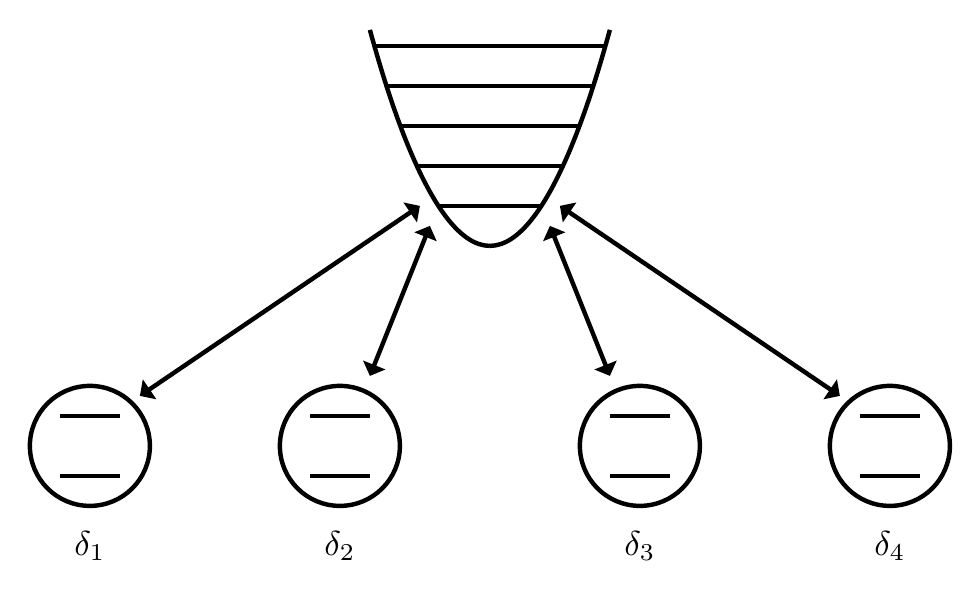
\begin{tikzpicture}[x=1.0in,y=1.0in]
    \draw[color=black!100 , ultra thick] (0,0) parabola (0.6,1.08) ;
    \draw[color=black!100 , ultra thick] (0.0,0.0) parabola (-0.6,1.08) ;
    \draw[color=black!100 , ultra thick] (-0.36514837167011072,.4) -- (0.36514837167011072,.4);
    \draw[color=black!100 , ultra thick] (0.2581988897471611,.2) -- (-0.2581988897471611,.2);
    \draw[color=black!100 , ultra thick] (0.44721359549995793,.6) -- (-0.44721359549995793,.6);
    \draw[color=black!100 , ultra thick] (0.5163977794943222,.8) -- (-0.5163977794943222,.8);
    \draw[color=black!100 , ultra thick] (0.57735026918962573,1.0) -- (-0.57735026918962573,1.0);
    \draw[color=black!100, ultra thick](-.75,-1) circle (.3);
    \node at (-.75 , -1.5){\scalebox{1.25}{$\delta_2$}} ;
    \draw[color=black!100, ultra thick](.75,-1) circle (.3);
    \node at (.75 , -1.5){\scalebox{1.25}{$\delta_{3}$}} ;
    %\draw[dotted , ultra thick] (.25,-1) -- (-.25,-1);
    \draw[color= black!100 , ultra thick] (-.6,-1.15)--(-0.9,-1.15);
    \draw[color= black!100 , ultra thick] (-.6,-.85)--(-0.9,-0.85);
    \draw[color= black!100 , ultra thick] (.6,-1.15)--(0.9,-1.15);
    \draw[color= black!100 , ultra thick] (.6,-.85)--(0.9,-0.85);
    \draw[color= black!100 , ultra thick] (-1.85,-1.15)--(-2.15,-1.15);
    \draw[color= black!100 , ultra thick] (-1.85,-.85)--(-2.15,-0.85);
    \draw[color= black!100 , ultra thick] (1.85,-1.15)--(2.15,-1.15);
    \draw[color= black!100 , ultra thick] (1.85,-.85)--(2.15,-0.85);
    \draw[color=black!100, ultra thick](-2,-1) circle (.3);
    \node at (-2.0 , -1.5){\scalebox{1.25}{$\delta_1$}} ;
    \draw[color=black!100, ultra thick](2,-1) circle (.3);
    \node at (2.0 , -1.5){\scalebox{1.25}{$\delta_{4}$}} ;
    \draw[black, ultra thick , tipA-tipA] (-0.6,-.65) -- (-0.3,0.1);
    \draw[black, ultra thick , tipA-tipA] (0.6,-.65) -- (0.3,0.1);
    \draw[black, ultra thick , tipA-tipA] (1.75,-.75) -- (0.35,0.2);
    \draw[black, ultra thick , tipA-tipA] (-1.75,-.75) -- (-0.35,0.2);
    \end{tikzpicture}
}

\subfigure[]{
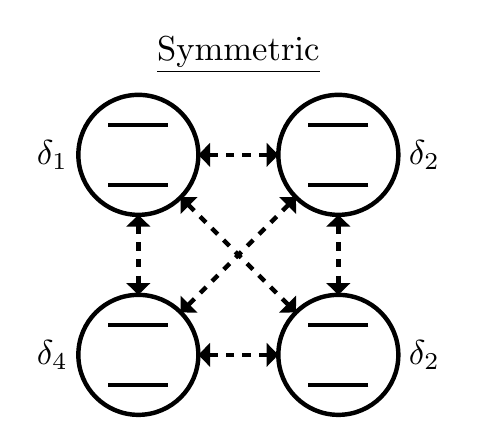
\begin{tikzpicture}[x=1.0in,y=1.0in]
\draw[color=black!100, ultra thick](.5,.5) circle (.3);
\node at (-0.93 , 0.5){\scalebox{1.25}{$\delta_1$}} ;
\draw[color=black!100, ultra thick](.5,-.5) circle (.3);
\node at (0.93 , 0.5){\scalebox{1.25}{$\delta_2$}} ;
\draw[color=black!100, ultra thick](-.5,.5) circle (.3);
\node at (-0.93 , -0.5){\scalebox{1.25}{$\delta_4$}} ;
\draw[color=black!100, ultra thick](-.5,-.5) circle (.3);
\node at (0.93 , -0.5){\scalebox{1.25}{$\delta_2$}} ;
\draw[dashed , ultra thick , tipA-tipA] (.2,.5) -- (-.2,.5);
\draw[dashed , ultra thick , tipA-tipA] (.2,-.5) -- (-.2,-.5);
\draw[dashed , ultra thick , tipA-tipA] (.5,.2) -- (.5,-.2);
\draw[dashed , ultra thick , tipA-tipA] (-.5,.2) -- (-.5,-.2);
\draw[color= black!100 , ultra thick] (.65,.35)--(.35,.35);
\draw[color= black!100 , ultra thick] (.65,.65)--(.35,.65);
\draw[color= black!100 , ultra thick] (-.65,.35)--(-.35,.35);
\draw[color= black!100 , ultra thick] (-.65,.65)--(-.35,.65);
\draw[color= black!100 , ultra thick] (.65,-.35)--(.35,-.35);
\draw[color= black!100 , ultra thick] (.65,-.65)--(.35,-.65);
\draw[color= black!100 , ultra thick] (-.65,-.35)--(-.35,-.35);
\draw[color= black!100 , ultra thick] (-.65,-.65)--(-.35,-.65);
\draw[dashed , ultra thick , tipA-tipA] (-.2878679656440358,-.2878679656440358)--(.2878679656440358,.2878679656440358);
\draw[dashed , ultra thick , tipA-tipA] (.2878679656440358,-.2878679656440358)--(-.2878679656440358,.2878679656440358);
\node at (0, 1.0){\underline{\scalebox{1.25}{Symmetric}}} ;
\end{tikzpicture}
}\hspace{3cm}
\subfigure[]{
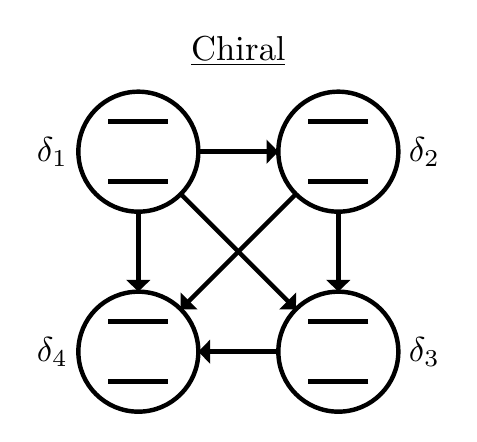
\begin{tikzpicture}[x=1.0in,y=1.0in]
\draw[color=black!100, ultra thick](.5,.5) circle (.3);
\node at (-0.93 , 0.5){\scalebox{1.25}{$\delta_1$}} ;
\draw[color=black!100, ultra thick](.5,-.5) circle (.3);
\node at (0.93 , 0.5){\scalebox{1.25}{$\delta_2$}} ;
\draw[color=black!100, ultra thick](-.5,.5) circle (.3);
\node at (-0.93 , -0.5){\scalebox{1.25}{$\delta_4$}} ;
\draw[color=black!100, ultra thick](-.5,-.5) circle (.3);
\node at (0.93 , -0.5){\scalebox{1.25}{$\delta_3$}} ;
\draw[ ultra thick , tipA-] (.2,.5) -- (-.2,.5);
\draw[ ultra thick , -tipA] (.2,-.5) -- (-.2,-.5);
\draw[ ultra thick , -tipA] (.5,.2) -- (.5,-.2);
\draw[ ultra thick , -tipA] (-.5,.2) -- (-.5,-.2);
\draw[color= black!100 , ultra thick] (.65,.35)--(.35,.35);
\draw[color= black!100 , ultra thick] (.65,.65)--(.35,.65);
\draw[color= black!100 , ultra thick] (-.65,.35)--(-.35,.35);
\draw[color= black!100 , ultra thick] (-.65,.65)--(-.35,.65);
\draw[color= black!100 , ultra thick] (.65,-.35)--(.35,-.35);
\draw[color= black!100 , ultra thick] (.65,-.65)--(.35,-.65);
\draw[color= black!100 , ultra thick] (-.65,-.35)--(-.35,-.35);
\draw[color= black!100 , ultra thick] (-.65,-.65)--(-.35,-.65);
\draw[ ultra thick , tipA-] (-.2878679656440358,-.2878679656440358)--(.2878679656440358,.2878679656440358);
\draw[ ultra thick , tipA-] (.2878679656440358,-.2878679656440358)--(-.2878679656440358,.2878679656440358);
\node at (0, 1.0){\underline{\scalebox{1.25}{Chiral}}} ;
\end{tikzpicture}
}
\caption{Four qubits coupled to a mutually shared resonator mode, with an associated detuning pattern $( \delta_1 , \delta_2 , \delta_3 , \delta_4)$. (b) In the symmetric scheme all qubits are coupled to each other through a dissipative coupling. (c) Addition of qubit-qubit couplings, and their interference with the dissipative couplings, renders all pairwise couplings in the chain unidirectional, such that the qubits on the left cannot ``see" the qubits to their right.}
\end{figure}
%
Consider a chain of four qubits interacting with a mutual resonator, as depicted in  system Fig. \ref{Fig:Detuning Pattern}(a). We assume homogeneous couplings, $g_i=g$, so
%
\begin{equation}
    \frac{H_{SR}'}{\hbar} = g b^\dagger ( \sigma_1 + \sigma_2 + \sigma_3 + \sigma_4) + h.c.
\end{equation}
%
Using the adiabatic elimination of the resonator, as described in the previous chapter, this allows a straightforward identification of the effective junp operator
%
\begin{eqnarray}
    \hat{S} = g ( \sigma_1 + \sigma_2 + \sigma_3 + \sigma_4)
\end{eqnarray}
%
which leads to the following master equation for the reduced system
%
\begin{equation}\label{four qubit}
    \dot{\rho}_S = - \frac{i}{\hbar} [H_S' , \rho_S] + \Gamma \mathcal{L}[\sigma_1 + \sigma_2 + \sigma_3 + \sigma_4] \rho_S.
\end{equation}
%
As before, $\Gamma = \frac{4g^2}{\kappa}$ is the engineered dissipation rate. Associated with each of the qubits is a detuning, $\delta_\alpha$, also depicted in in Fig. \ref{Fig:Detuning Pattern}(a). These detunings must come in equal and opposite pairs to form a perfectly coherent emitter-absorber with no spontaneous emission into the guided mode \cite{Cascade_Quantum_Systems}. That is for each qubit $j$ with a detuning $\delta_j$, there is another qubit $l$ in the chain with $\delta_j = - \delta_l$. 
%
\par
%
We will again consider the stabilization dynamics for both:
%
\begin{itemize}
\item a symmetric interaction between each pair of qubits, for which the qubit Hamiltonian is invariant under pairwise permutations [Fig. \ref{Fig:Detuning Pattern}(b)],
\begin{equation}
    H_{sym} = \sum_i \left( \frac{\delta_i}{2} \sigma_{zi} + \frac{\Omega}{2} \sigma_{xi} \right)
\end{equation}
\item a chiral interaction between each pair of qubits, for which the qubit Hamiltonian is no longer invariant under pairwise permutations [Fig. \ref{Fig:Detuning Pattern}(c)],
\begin{equation}
   H_{chiral} = H_{sym} - i \frac{\Gamma}{2} \sum_{i > j} \left( \sigma_j^\dagger \sigma_i - \sigma_j \sigma_i^\dagger \right)
\end{equation}
This is because the qubit-qubit couplings pick up a phase under an index swap. Recall that the combination of these couplings with engineered dissipation creates unidirectional emission and absorption from left-to-right in the chain, as demonstrated for the Bell state stabilization in the last chapter.
\end{itemize}
%
%
%We will find that the detuning pattern will determine whether four-way entanglement arises in the qubits space. First we will show how the purity of qubit subspace can be used to determine entanglement. Finally we will consider entanglement in the symmetric and chiral stabilization scheme. 
%
%The asymmetric part is responsible qubit-qubit couplings so that the net driven-dissipative interaction is chiral. Each of the qubits is driven symmetrically that is $\Omega_i = \Omega$. Furthermore the detunings between qubit pairs that chancel out so that for every qubit qubit $i$ in the chain with a detuning $\delta_i$ there is another qubit $l$ in the chain with a detuning that satisfies $\delta_i = - \delta_l$. When these conditions are satisfied the qubit chain will dimeraterize. That is the steady state of the qubit chain can be in terms of different dimers
%
\section{Role of chirality}
%
We consider the entanglement dynamics in the symmetric and chiral case for two different types of detuning patterns: alternating and staggered. An alternating detuning pattern is of the form $(\delta_a , - \delta_a , \delta_b , - \delta_b )$. A staggered detuning is obtained by permuting two of the detunings: $(\delta_a , \delta_b , -\delta_a , - \delta_b )$.
%
\par
%
\subsection{Entanglement Identification}
%
In order to identify the nature of multipartite entanglement in each case, we use a quantity called the purity of the density matrix: $tr
\left( \rho^2 \right)$. The purity of the density matrix has the following property
 \begin{eqnarray}
 tr( \rho^2 ) & = & 1 \quad\text{ for a pure state} \nonumber \\
  tr( \rho^2 ) & < & 1 \quad\text{ for a mixed state}. \nonumber
 \end{eqnarray}
Now suppose two subsystem in the chain are entangled. Then by definition the total state, $| \Phi \rangle$, cannot written as a product state of the two subsystems. That is 
 \begin{equation}
 |\Phi \rangle \neq |\phi_1 \rangle \otimes |\phi_2 \rangle.
 \end{equation}
 Therefore when one of the subsystems is traced over, the resulting density matrix is mixed with a purity less than one \cite{Entangle_Time_Scale}. For example, suppose two qubits $j$ and $k$ in the chain are entangled.
\begin{equation}
| S \rangle_{j k } = \frac{1}{\sqrt{2}} \left( | g e \rangle_{j k } - | e g \rangle_{ j k } \right)
\end{equation}
We trace over the subspace $j$ and find
\begin{equation}
    \rho_{k} = tr_j \lbrace | S \rangle_{j k }\langle S | \rbrace = \frac{1}{2} \left(| e \rangle_k \langle e | + | g \rangle_k \langle g |\right) = \frac{1}{2} \left( \begin{array}{cc}
       1  & 0 \\
       0  & 1
    \end{array} \right).
\end{equation}
Computing $tr_k \left\lbrace \rho_k^2 \right\rbrace = 0.5 < 1 $, we see that the subsystem is mixed and its purity is less than one.
%
\subsection{Alternating Detunings}
%
The results for purity plots are shown in Fig. \ref{fig:alternating}. Our results show that both the symmetric and chiral schemes purify the state $|S\rangle_{12} | S \rangle_{34}$. However, the chiral purification is faster by more than a factor of 10. Furthermore, in the chiral case $|S\rangle_{12}$ is stabilized before $|S\rangle_{34}$ displaying the system's unidirectional nature.
%
\begin{figure}[t!]
%    \textbf{$\Gamma= 4\frac{g^2}{\kappa}=10 \; \delta_a = 1 \; \delta_b = 4 , \Omega=8$}\par
%    \textbf{$(\delta_a , - \delta_a , \delta_b , - \delta_b )$}\par
\centering
\subfigure[]{
  \includegraphics[scale=.85]{Images/Sym_Alternating.pdf}
}
\vspace{-.5cm}
\subfigure[]{
  \includegraphics[scale=.85]{Images/Chiral_Alternating.pdf}
}
%\vspace{3mm}
    \caption{Time-domain simulations of a four-qubit chain for symmetric and chiral cases with alternating detuning pattern: $(\delta_a , - \delta_a , \delta_b , - \delta_b )$. All the plots were generated with the same parameters, $\Gamma= 4\frac{g^2}{\kappa}=10, \; \delta_a = 1, \; \delta_b = 4, \; \Omega=8$.}
    \label{fig:alternating}
\end{figure}
%
%
\subsection{Staggered Detunings}
%
The results for purity plots are shown in Fig. \ref{fig:staggered}. For the symmetric coupling case we get non-local (though still pairwise) entanglement, and the state $|S\rangle_{13}|S\rangle_{24}$ is purified. However, for chiral couplings, only the full 4-qubit system purity goes to one indicating that the steady state exhibits genuine four-qubit entanglement. 
%
\begin{figure}[h!]
%\textbf{$\Gamma= 4\frac{g^2}{\kappa}=10 \; \delta_a = 1 \; \delta_b = 4 , \Omega=8$}\par
%    \textbf{$(\delta_a , - \delta_a , \delta_b , - \delta_b )$}\par
\centering
\subfigure[]{
  \includegraphics[scale=.85]{Images/Sym_Staggered.pdf}
}
\vspace{-.5cm}
\subfigure[]{
  \includegraphics[scale=.85]{Images/Chiral_Staggered.pdf}
}
%\vspace{3mm}
    \caption{Time-domain simulations of a four-qubit chain for symmetric and chiral cases with staggered detuning pattern, $(\delta_a , \delta_b , - \delta_a , - \delta_b )$. All the plots were generated with the same parameters, $\Gamma= 4\frac{g^2}{\kappa}=10, \; \delta_a = 1, \; \delta_b = 4, \; \Omega=8$.}
    \label{fig:staggered}
\end{figure}
%
\section{Caveat: Symmetric Four-qubit Entanglement}
%
Consider the homogeneous detuning detuning pattern
\begin{equation}\label{Detuning_Pattern}
 ( \delta ,  \delta , -\delta , - \delta  ).
\end{equation}
The third and fourth qubit can both form a coherent emitter-absorber pair with the first qubit because the detunings are equal and opposite. In other words, the first qubit can become entangled with the third qubit or the forth qubit. Because there can be no preferred entangled state, we found that the steady state was a superposition of the two possible configurations. Thus the detuning pattern, Eq. (\ref{Detuning_Pattern}), stabilizes
\begin{equation}
 \frac{1}{\sqrt{2}}\left( | S \rangle_{13} | S \rangle_{24} + | S \rangle_{14} | S \rangle_{23} \right).
\end{equation}
However, for this scheme to work the system has to be initialized in the ground state,  i.e.
\begin{equation}
    \rho_S(0) = | gggg \rangle \langle gggg |.
\end{equation}
We found a significant decrease in steady state fidelity when intialized in a mixed state. Table 4.1 summarizes the different permutations of the detuning pattern and the corresponding four-qubit entangled states that get stabilized as a result.
%
\begin{table}[t!]\label{Bell State Table}
\centering
\begin{tabular}{c|c}
\centering
Detuning Pattern & Stabilized State \\
\hline
$( \delta , - \delta , \delta , - \delta  )$ & $| S \rangle_{12} | S \rangle_{34} - | S \rangle_{14} | S \rangle_{23}$  \\
$( \delta , - \delta , -\delta ,  \delta  )$ & $ | S \rangle_{12} | S \rangle_{34} + | S \rangle_{13} | S \rangle_{24}$  \\
$( \delta , \delta , - \delta , - \delta  )$  & $ | S \rangle_{13} | S \rangle_{24} + | S \rangle_{14} | S \rangle_{23}$ 
\end{tabular}
\caption{Table of detuning patterns and corresponding stabilized four-qubit entangled state).}
\end{table}
%
\begin{figure}[h!]
\centering
%    \textbf{$\Gamma= 4\frac{g^2}{\kappa}=10 \; \delta = 1 \; \Omega=8$}\par
\includegraphics[scale=.85]{Images/Sym_Homo.pdf}
    \caption{Purity plots show that the steady state is a four-qubit entangled state when the system is initialized in the ground state, and the detuning pattern is homogeneous. The parameters used for the simulation were $\Gamma= 4\frac{g^2}{\kappa}=10, \; \delta = 1, \; \Omega=8$.}
    \label{fig:}
\end{figure}

% Chapter 4: Conclusions
%-------------------------------------------------------------
\chapter{Conclusion}

In conclusion, we have shown that even though dissipation can lead to decohernce that washes away quantum information, it possible to use dissipation to our advantage to stabilize entanglement with high-fidelity. Specifically, we presented schemes for two- and four-qubit entanglement generation, employing an ``engineered" qubit-reservoir coupling. The reservoir in question can be implemented via a lossy harmonic oscillator. Such a scheme is compatible with standard circuit-QED platforms using microwave resonators and superconducting qubits. 

We showed how the method of adiabatic elimination provides a convenient route to identify ``engineered" jump operator that captures the effective dissipation seen by the qubits. This allows us to study open system dynamics of only the reduced system of interest, giving considerable advantage in terms of both analytical tractability and numerical computation. We found that for parameters considered here, entanglement stabilization with chiral qubit interactions outperforms the scheme that relies on symmetric qubit interactions. This was quantified in terms of a new performance metric $M$: realizing a large value of this metric entails a \emph{simultaneous} maximization of fidelity and rate of stabilization. The chiral scheme had a performance metric that was 10x bigger than the symmetric scheme for optimal parameters. 

Furthermore, four-qubit studies show that chirality is essential to purify mixtures into genuine multipartite entangled states. The `knob' that determines the nature of entanglement in a 1D chiral qubit chain is the detuning pattern of the driving field: if the detunings are ``alternating" the qubits stabilize into pairs of singlets, while when the detunings are ``staggered" (realized by permuting one of the detunings), the steady state is a true tetramer. Multipartite entanglement stabilization may be possible from symmetric dissipative interactions alone, but this requires specific driving conditions along with initial state preparation. We also find that the time scales and dynamics in qubits chains are qualitatively different with and with out chirality, which will form the basis of future investigations.

%In this thesis we have have considered the dynamics of dissipative engineering protocols and shown that multi-qubit entanglement is possible when coupled to a low Q-value cavity mode. These schemes always requires a strong resonate drive and display a trade off between fidelity and gap. However, the addition of chiral coupling seems to make the overall stabilization scheme better. Furthermore, chiral couplings are necessary for the purification of a four way entangled. 

%Finally, I would like to discuss future directions that this research can go. Also like to discuss how our work fits in with the broader field of chiral quantum optics. While in this thesis we considered qubits coupled to a mutual cavity mode one could consider qubits/spins coupled to a chiral wave-guide (see Appendix). Spins coupled to a chiral wave-guide have applications quantum communication protocols. One possibly is quantum state transfer (\cite{QuNoise}})


\appendix
% Appendix
%-------------------------------------------------------------
%
%ccccccccccccccccccccccccccccccccccccccccccccccc
\chapter{Rotating Frames}\label{Rotating Frame}
%ccccccccccccccccccccccccccccccccccccccccccccccc
%
Let us start with the Schrodinger equation in a stationary frame
\begin{equation}\label{Stationary_Frame_Schrodinger_Equation}
i \hbar \frac{d}{dt} \left| \Psi \> = H \left| \Psi \>.
\end{equation}
we desire to transform it into a rotating frmae using a unitary operator of the form
\begin{equation}
\hat{U} = \exp\left( i \hat{G} t / \hbar \right),
\end{equation}
with $\hat{G}$ clearly being self-adjoint. We now define the rotating state vector
\begin{equation}\label{Rotating_Frame_State_Vector}
| \tilde{\Psi} \rangle = \hat{U} \left| \Psi \>.
\end{equation}
We now need to find the  transformed Hamiltonian $\tilde{H}$ by constructing the Schrodinger Equation in a rotating frame. To this end, we substitute Eq. (\ref{Rotating_Frame_State_Vector}) in Eq. (\ref{Stationary_Frame_Schrodinger_Equation})
\begin{eqnarray}\label{Tranforming_Into_Rotating_Frame}
i\hbar \frac{d}{dt} \left( \hat{U}^\dagger | \tilde{\Psi} \rangle \right) & =& H \hat{U}^\dagger | \tilde{\Psi} \rangle \nonumber \\
i\hbar \hat{U}^\dagger \frac{d}{dt} | \tilde{\Psi} \rangle  + i \hbar \frac{d\hat{U}^\dagger}{dt} | \tilde{\Psi_R} \rangle & = & H \hat{U}^\dagger | \tilde{\Psi} \rangle \nonumber \\
\hat{U}^\dagger \left(i \hbar \frac{d}{dt} | \tilde{\Psi} \rangle \right) & = &  H \hat{U}^\dagger | \tilde{\Psi} \rangle - i \hbar \frac{d \hat{U}^\dagger}{dt} | \tilde{\Psi} \rangle \nonumber \\
i \hbar \frac{d}{dt} | \tilde{\Psi} \rangle & = & \left( \hat{U} H \hat{U}^\dagger - i \hbar \hat{U}\frac{d \hat{U}^\dagger}{dt}  \right) | \tilde{\Psi} \rangle.
\end{eqnarray}
Comparing the Schrodinger Equation in a rotating frame 
\begin{equation}
i \hbar \frac{d}{dt} | \tilde{\Psi} \rangle = \tilde{H} | \tilde{\Psi} \rangle
\end{equation}
to Eq. (\ref{Tranforming_Into_Rotating_Frame}) we conclude that the rotating frame Hamiltonian is 
\begin{equation}
\tilde{H} =\hat{U} H \hat{U}^\dagger - i \hbar \hat{U}\frac{d \hat{U}^\dagger}{dt} =  \hat{U} H \hat{U}^\dagger - \hat{G}. 
\end{equation}




%
%ccccccccccccccccccccccccccccccccccccccccccccccccc
\chapter{Superoperator Algebra}\label{Super Operator Algebra}
%ccccccccccccccccccccccccccccccccccccccccccccccc
%
Superoperators act on operators to produce new operators, just as operators act on vectors to produce new vectors. The key difference is that superoperators ``embrace" their arguments. How they are embraced is conveyed using a dot notation.
\begin{equation}
\left( a^{\dagger 2} b \bullet \right) \hat{O} \equiv a^{\dagger 2} b \hat{O} \qquad \left(a \bullet a^{\dagger} \right) \hat{O} \equiv a \hat{O} a^{\dagger} \qquad \left( \bullet b^{\dagger} b \right) \hat{O} \equiv \hat{O} b^{\dagger} b.
\end{equation}

Superoperator products are evaluated by substituting the superoperator, on the right, where the dot is, on the left.
\begin{equation}
 \left( a^{\dagger 2} \bullet \right) \left( b \bullet \right) = \left( a^{\dagger 2} b \bullet \right) \qquad \left( a \bullet \right)\left( \bullet a^{\dagger} \right) = \left( a \bullet a^{\dagger} \right) \qquad \left( \bullet b \right) \left( \bullet b^{\dagger} \right) = \left( \bullet b^{\dagger} b \right)
\end{equation}
It is also possible to work in the reverse direction and ``factorize" a superoperator into products.

In general two superoperators do not commute. However, if every operators in a superoperators commutes with every operator in another superoperator then the superoperators commute. For example
\begin{eqnarray}
\left( a \bullet a^{\dagger} \right)\left( b \bullet b^{\dagger} \right) & = & \left( ab \bullet b^{\dagger} a^{\dagger} \right) = \left( b a \bullet a^{\dagger} b^{\dagger} \right) \nonumber \\
& = & \left( b \bullet b^{\dagger} \right) \left( a \bullet a^{\dagger} \right).
\end{eqnarray}

Given a superoperators $S$, we associate with it a conjugate superoperator, $S^{\dagger}$. Consider
\begin{equation}
\left( S \hat{O} \right)^{\dagger} \equiv S^{\dagger} \hat{O}^{\dagger} = S^{\dagger} \hat{O}
\end{equation}
where the operator $\hat{O}$ is assumed to be hermitian because $\hat{O}$ will typically be a density operator. Consider the example
\begin{eqnarray}
\left( \left( a^{\dagger 2 } b \bullet \right) \hat{O} \right)^{\dagger} & = & \left( a^{\dagger 2 } b \hat{O} \right)^{\dagger} = \left( \hat{O}^{\dagger} b^{\dagger} a^{2} \right) \nonumber \\
& = & \left( \bullet b^{\dagger} a^{2} \right) \hat{O}
\end{eqnarray}
thus
\begin{equation}
\left( a^{\dagger 2 } b \bullet \right)^{\dagger} = \left( \bullet b^{\dagger} a^2 \right).
\end{equation} 
We can write the above equation in the form
\begin{equation}
\left[ \left( a^{\dagger 2 } \bullet \right) \left( b \bullet \right) \right]^{\dagger} = \left[ \left( \bullet a^2 \right) \left( \bullet b^{\dagger} \right) \right]
\end{equation}
from which we conclude
\begin{equation}\
\left( S_1 S_2 \right)^{\dagger} = S_1^{\dagger} S_2^{\dagger}.
\end{equation}
Therefore the ordering of the superoperators does not change when the hermitian conjugate is taken.

We now will move on to calculating commutators of superoperators. Consider
\begin{eqnarray}
\left[ \left( b \bullet b^{\dagger} \right) , \left( b \bullet \right) \right] =  \left( b \bullet b^{\dagger} \right) \left( b  \bullet \right) - \left( b \bullet \right) \left( b \bullet b^{\dagger} \right) = 0  \nonumber \\
\end{eqnarray}
and
\begin{eqnarray}
\left[ \left( b^{\dagger} b \bullet \right) , \left( b \bullet \right) \right] & = & \left( b^{\dagger} b \bullet \right)\left( b \bullet \right) - \left( b \bullet \right) \left( b^{\dagger} b \bullet \right) \nonumber \\
& = & \left( b^{\dagger} b^2 \bullet \right) - \left( b b^{\dagger} b \bullet \right) \nonumber \\
& = & \left( b^{\dagger} b \bullet - b b^{\dagger} \bullet \right) \left( b \bullet \right) \nonumber \\ 
& = & - \left( b \bullet \right). \nonumber 
\end{eqnarray}

A time dependent operator of the form satisfies 
\begin{equation}
S'(t) \equiv e^{- \mathcal{L} t } S e^{ \mathcal{L} t }
\end{equation}
obey's the Heisenberg equation of motion
\begin{equation}
\frac{d}{d t } S'(t) = \left[ S', \mathcal{L} \right].
\end{equation}
We now will solve the equation of motion. Consider $\mathcal{L}= \kappa \left( 2 b \bullet b^{\dagger} - b^{\dagger} b \bullet - \bullet b^{\dagger} b \right)$ and $S'(0)=\left( b \bullet \right)$.
\begin{eqnarray}
\frac{d}{d t}\left( b \bullet \right)' & = & \kappa \left[ \left(b\bullet\right)', 2\left(b \bullet b^{\dagger} \right)' - \left( b^{\dagger} b \bullet \right)' - \left( \bullet b^{\dagger} b \right)' \right] \nonumber \\
& = & - \kappa \left( b \bullet \right)'
\end{eqnarray}
which has a solution of the form
\begin{equation}
S'(t) = (b \bullet)' = e^{- \mathcal{L} t } \left( b \bullet \right) e^{ \mathcal{L} t}= e^{ - \kappa t }\left( b \bullet \right).
\end{equation}
This example is simple because the superoperator $\left( b \bullet \right)'$ does not couple to other superoperators. However, in the following example $\left( b^{\dagger} \bullet \right)$ couples to $\left( \bullet b^{\dagger} \right)$.
\begin{eqnarray}
\frac{d}{d t } \left( b^{\dagger} \bullet \right)' & = & \left[ \left( b^{\dagger} \bullet \right)' , 2 \left( b \bullet b^{\dagger} \right)' - \left( b^{\dagger} b \bullet \right)' - \left( \bullet b^{\dagger} b \right)' \right] \nonumber \\
 & = & \kappa \left( b^{\dagger} \bullet \right)' - 2 \kappa \left( \bullet b^{\dagger} \right)' \\
\frac{d }{d t } \left( \bullet b^{\dagger} \right) & = & \kappa \left[ \left( \bullet b^{\dagger} \right)', 2 \left( b \bullet b^{\dagger} \right)' - \left( b^{\dagger} b \bullet \right)' - \left( \bullet b^{\dagger} b \right)' \right] = - \kappa \left( \bullet b^{\dagger} \right)' 
\end{eqnarray}
The solution to equation Eq. (14) can be found by substituting $\left( \bullet b^{\dagger} \right)'=\left( \bullet b^{\dagger}\right)e^{-\kappa t}$. plugging in this solution into equation (13) the solution becomes
\begin{equation}
\left( b^{\dagger} \bullet \right)' = \left( \bullet b^{\dagger} \right) \left( e^{-\kappa t} - e^{\kappa t} \right) + \left( b^{\dagger} \bullet \right) e^{\kappa t}.
\end{equation}


%Evaluating commutator the equations of motion are
%\begin{eqnarray}
%\frac{d }{d t } \mathcal{R}_1'(t) & = & \frac{d}{d t}(b \bullet )' = [b \bullet , \mathcal{L}_R ] = \left( -i \Delta - \frac{\kappa}{2} \right) \left( b \bullet \right) \nonumber \\
%\frac{d}{d t} \mathcal{R}_1'^{\dagger}(t) &=&  \frac{ d }{d t }\left( \bullet b^{\dagger} \right)' = [ \bullet b^{\dagger} , \mathcal{L}_R ] = \left( i \Delta - \frac{\kappa}{2} \right) \left(\bullet b^{\dagger} \right) \nonumber \\
%\frac{d }{d t } \mathcal{R}_2'(t) & = & \frac{d }{d t} \left( b^{\dagger} \bullet \right) =  [b^{\dagger} \bullet , \mathcal{L}_R] = \left( i \Delta + \frac{\kappa}{2} \right) \left( b^{\dagger} \bullet \right) - \kappa \left( \bullet b^{\dagger} \right) \nonumber \\
%\frac{d}{d t } \mathcal{R}_2'^{\dagger} (t)  & = & \frac{d}{dt }\left( \bullet b \right)' = \left( - i \Delta + \frac{\kappa}{2} \right) \left( \bullet b \right) - \kappa \left( b \bullet \right)  \nonumber
%\end{eqnarray}


\chapter{Parametric Interactions: Stabilizing Arbitray Bell States}

Two spins coupled to a mutual cavity mode can in principle stabilize any of the following bell states
\begin{eqnarray}
\left| S \> & = &  \frac{1}{\sqrt{2}} \left( \left| g e \> - \left| e g\> \right) \nonumber \\
\left| T \> & = &  \frac{1}{\sqrt{2}} \left( \left| g e \> + \left| e g\> \right) \nonumber \\
\left| \Phi_- \> & = &  \frac{1}{\sqrt{2}} \left( \left| e e \> - \left| g g\> \right) \nonumber  \\
\left| \Phi_+ \> & = &  \frac{1}{\sqrt{2}} \left( \left| e e \> + \left| g g\> \right) \nonumber 
\end{eqnarray} 
for a strong resonate drive. However, these states all belong to the null space of a different jump operator. For example, $(\sigma_1 - \sigma_2)|T\rangle = 0 $. Because there is a phase difference between $\sigma_1$ and $\sigma_2$ in the jump operator, there needs to be a phase difference between the couplings strength. That is $g_1 = - g_2 = g$, so $\frac{H_{SR}}{\hbar} = b^\dagger(g_1 \sigma_1 + g_2 \sigma_2 ) = g b^\dagger \left( \sigma_1 - \sigma_2\right)$.

To stabilize the states $\left| \Phi_- \>$ the operator $\sigma_2 \longrightarrow \sigma_2^\dagger$, so $(\sigma_1 + \sigma_2^\dagger)| \Phi_- \rangle = 0 $. This means system-reservoir interaction Hamiltonian must have the form post RWA
\begin{equation}\label{Phi_minus_Hamiltonian}
\frac{H_{SR}'}{\hbar} \approx g_2 b^\dagger( \sigma_1 + \sigma_2^\dagger) + h.c. 
\end{equation}
The system-resvoir coupling for the second qubit has now becomes an amplification Hamiltonian.
\begin{equation}
H_{SR}^{(2)} \approx g_2 b^\dagger \sigma_2^\dagger + h.c.
\end{equation}
To get an amplification Hamiltonian from the lab frame Hamiltonian, Eq. (\ref{Two Quipt Pamametric Couplings}), the static coupling $g_2$ must become a ``parametric" time-dependent coupling. That is
\begin{equation}
    g_2 \rightarrow g_2(t) = g_2 e^{i \omega_{p2} t} + c.c.
\end{equation}
When we move into the rotating frame, as defined in Eq. (\ref{Equ:Rotating_Hamiltonian}), we pick the modulation frequencies to be the sum $\omega_{p2} = \omega_2 + \omega_c$. After RWA the resulting Hamiltonian is Eq. (\ref{Phi_minus_Hamiltonian}). To stabilize $|\Phi_+\rangle$ we make sure $g_1=-g_2 =g$ so the effective jump operator satisfies $(\sigma_1 - \sigma_2^\dagger)| \Phi_+ \rangle = 0$.

\begin{table}\label{Bell State Table}
\centering
\begin{tabular}{c|c}
\centering
Bell State & Engineered Jump Operator \\
\hline
$\left| S \>$ & $\sigma_1 + \sigma_2$  \\
$\left| T \>$ & $\sigma_1 - \sigma_2$  \\
$\left| \Phi_- \>$  & $\sigma_1 + \sigma_2^\dagger$ \\
$\left| \Phi_+ \>$  & $\sigma_1 - \sigma_2^\dagger$ 
\end{tabular}
\caption{Table of bell states with corresponding jump operator. One can easily verify that the bell state is part null space the corresponding jump operator.}
\end{table}

%\section{Spins Coupled to a Wave-Guide}

%Consider the total Hamiltonian given by
%\begin{equation}\label{H_tot}
%H_{tot}=H_{sys} + H_{res} + H_{int}
%\end{equation}
%where
%\begin{equation}
%H_{sys}  =  \hbar \sum_{j=1}^{N} \left( - \delta_j \sigma_j^{\dagger} \sigma_j + \Omega \sigma_j + \Omega^* \sigma_j^{\dagger} \right) 
%\end{equation}
%\begin{equation}\label{H_bath}
%H_{res}  = \sum_{\lambda=L,R} \int d\omega \; \hbar \omega b_{\lambda}^{\dagger}( \omega ) b_{\lambda}( \omega )
%\end{equation}
%\begin{equation} \label{H_int}
%H_{int}  =  i \hbar \sum_{\lambda=L,R} \sum_{j=1}^{N} \int d \omega \sqrt{\frac{\gamma_{\lambda j }}{2 \pi }} b_{\lambda}^{\dagger}(\omega) \sigma_j e^{- i \left( \nu t + \omega x_j / v_\lambda \right)} + h.c.
%\end{equation}
%Defining a rotating frame $|\Psi_R\rangle = e^{i H_{res} t/\hbar } | \Psi \rangle$, that is moving into the interaction picture with respects to the bath Hamiltonian, the total Hamiltonian becomes
%\begin{equation}
%H_{tot}(t) = H_{sys} + e^{i H_{res} t/\hbar } H_{int} e^{- i H_{res} t/\hbar }.
%\end{equation}
%To evaluate the interaction term in the rotating frame the Baker-Hausdorff theorem along with the commutation relationship $[b_\lambda(\omega ) , b_{\lambda' } ( \omega ' ) ] = \delta_{\lambda \lambda'} \delta( \omega - \omega')$ can be used.  However this computation would be tedious so consider a simpler model where $H_B= \omega a^{\dagger} a$  and $H_I = ig \left( a^{\dagger} \sigma - a \sigma^{\dagger} \right)$. In the rotating frame the interaction becomes 
%\begin{equation}
%e^{ i H_B t } H_I e^{ - i H_B t } = ig \left( a^{\dagger} \sigma e^{i \omega t } - a \sigma^{\dagger} e^{-i \omega t } \right).
%\end{equation}
%Therefore in the rotating frame $a \rightarrow a^{- i \omega t }$ and $a^{\dagger} \rightarrow a^{\dagger} e^{i \omega t }$. Amusing that this prescription works in the continuous case the interaction Hamiltonian becomes
%\begin{eqnarray}
%H_{int}(t) & = & e^{i H_B t/\hbar } H_{int} e^{- i H_B t/\hbar } \nonumber \\
%& = &  i \hbar \dubsum \int d \omega \sqrt{\frac{\gamma_{\lambda j }}{2 \pi }} b_{\lambda}^{\dagger}(\omega) \sigma_j e^{- i \left( \left[ \nu - \omega \right] t + \omega x_j / v_\lambda \right)} + h.c.
%\end{eqnarray}
%where $b_\lambda(\omega) \rightarrow b_\lambda(\omega)^{- i \omega t }$ and $b_\lambda^{\dagger}(\omega ) \rightarrow b_\lambda^{\dagger}(\omega) e^{i \omega t }$ Thus the total Hamiltonian is
%\begin{equation} \label{H_tot_rot}
%H_{tot}(t) = H_{sys} +  i \hbar \dubsum \int d \omega \sqrt{\frac{\gamma_{\lambda j }}{2 \pi }} b_{\lambda}^{\dagger}(\omega) \sigma_j e^{- i \left( \left[ \nu - \omega \right] t + \omega x_j / v_\lambda \right)} + h.c.
%\end{equation}
%
%Defining time dependent operators for the bath as  $b_{\lambda} ( \omega , t ) = U^{\dagger}(t) b_{\lambda} (\omega) U(t)$ and $a( t ) = U^{\dagger}(t) a U(t)$ the Heisenberg Equation of can written as
%\begin{eqnarray}
%\dot{b}_{\lambda}(\omega, t) & = &U^{\dagger}(t)  [ b_{\lambda}(\omega) ,  H_{int}(t) ] U(t) \nonumber \\
%\dot{a} & = & \frac{1}{i \hbar} U^{\dagger}(t) [ a , H_{tot}(t) ] U(t)
%\end{eqnarray}
%where the unitaries satisfy $\dot{U}(t)  =  \frac{1}{i \hbar} H_{tot}(t) U(t)$ and $\dot{U}^{\dagger}(t) = - \frac{1}{i \hbar} U^{\dagger} ( t ) H_{tot}(t) $. Taking the time derivatives
%\begin{eqnarray}
%\dot{b}_{\lambda}(\omega, t) & = & \frac{1}{i \hbar} U^{\dagger}(t)  [ b_{\lambda}(\omega) , H_{tot}(t) ] U(t) =  \frac{1}{i \hbar} U^{\dagger}(t)  [ b_{\lambda}(\omega) ,  H_{int}(t) ] U(t) \nonumber \\
%& = & \sum_{\lambda'=R,L} \sum_{j=0}^N \int d \omega' \;  \sqrt{ \frac{\gamma_{\lambda' j } }{2 \pi } } U^{\dagger}(t) \underbrace{ [ b_\lambda(\omega) , b^{\dagger}_{\lambda'}( \omega') ] }_{\delta_{\lambda \lambda'} \delta( \omega - \omega') } \sigma_j U(t)e^{- i \left( \left[ \nu - \omega' \right] t + \omega' x_j / v_\lambda \right)} \nonumber \\
%& = & \sum_{j = 0 }^N \sqrt{\frac{\gamma_{\lambda l } }{2 \pi}} \sigma_j(t) e^{- i \left( \left[ \nu - \omega \right] t + \omega x_j / v_\lambda \right)} \nonumber \\
%\end{eqnarray}
%where $\sigma_j(t) = U^{\dagger}(t) \sigma_j U(t)$.
%The formal solution to this equation is
%\begin{equation}
%b_{ \lambda } ( \omega , t ) = b_{\lambda}(\omega) + \int_0^t ds \suml \sqrt{\frac{ \gamma_{\lambda l } }{2 \pi } } \sigma_l ( s ) e^{- i \left( \left[ \nu - \omega \right] s + \omega x_j / v_\lambda \right)}
%\end{equation}
%where the summation over $j$ has been replaced with a summation over $l$.
%
%Taking a time of system operator $a(t)$
%\begin{eqnarray}
%\dot{a}(t) & = &  \frac{1}{i \hbar} U^{\dagger}(t) [ A , H_{tot}(t) ] U(t) =  \frac{1}{i \hbar} U^{\dagger}(t) [ a , H_{sys} ] U(t) + \frac{1}{i \hbar} U^{\dagger}(t) [ a , H_{int}(t) ] U(t) \nonumber \\
%& = & - \frac{i}{\hbar} [ a(t) , H_{sys}(t) ]  \nonumber \\
%&+& \dubsum  \intw \sqrt{\frac{\gamma_{\lambda j }}{2 \pi }} \left( U^{\dagger}(t) b_{\lambda}^{\dagger}( \omega )[a , \sigma_j ] U(t)e^{  i ( ... )} - U^{\dagger}(t) b_\lambda(\omega) [ a , \sigma_j^\dagger ] U(t)e^{ -i ( ... ) } \right) \nonumber \\
%& = & - \frac{i}{\hbar} [ a(t) , H_{sys}(t) ] \nonumber \\
%& + & \dubsum  \intw \sqrt{\frac{\gamma_{\lambda j }}{2 \pi }} \left( b_{\lambda}^{\dagger}( \omega , t )[a(t) , \sigma_j(t) ]e^{ i ( ... )} - b_\lambda(\omega , t ) [ a(t) , \sigma_j^\dagger(t) ] e^{ - i ( ... ) } \right) \nonumber
%\end{eqnarray}
%where $g(t)=i ( \omega - \nu ) t - i \omega x_j/v_\lambda=i(\omega - \nu )(t - x_j / v_\lambda ) -  i \nu x_j / v_\lambda$. Substituting the formal solution into the above equation leads to
%
%\begin{align}
%\dot{a}(t) &= - \frac{i}{\hbar}[ a(t) , H_{sys}(t) ]  \\
%&\quad +  \dubsum \intw  \sqrt{\frac{\gamma_{\lambda j }}{2 \pi}} \left\lbrace [a(t) , \sigma_j(t) ]e^{i (...) }  \left[ b_{\lambda}^{\dagger}(\omega) + \int_0^t ds \suml \sqrt{\frac{ \gamma_{\lambda l } }{2 \pi } } \sigma_l^{\dagger} ( s ) e^{ i \left( \left[ \nu - \omega \right] s + \omega x_j / v_\lambda \right)}\right] \right]   .  \nonumber \\
%  &\quad \left. -   [ a(t) , \sigma_j^{\dagger}(t) ]e^{ - i (...)} \left[b_{\lambda}(\omega) + \int_0^t ds \suml \sqrt{\frac{ \gamma_{\lambda l } }{2 \pi } } \sigma_l ( s ) e^{- i \left( \left[ \nu - \omega \right] s + \omega x_j / v_\lambda \right)} \right] \right\rbrace.  \nonumber 
%\end{align}
%Distributing $\intw$ and $e^{-i (.. )}$ then defining defined the quantum noise operators $b_\lambda(t) = \frac{1}{2 \pi }\int d \omega b_\lambda ( \omega ) e^{- i ( \omega - \nu ) t }$ then
%\begin{eqnarray}
%\intw b_\lambda( \omega ) e^{-i (...) } & = & e^{ i \nu x_j / v_\lambda }\intw b_{\lambda}^{\dagger} ( \omega ) e^{ - i \left( \omega - \nu \right) \left( t - x_j/v_\lambda\right) } = \sqrt{ 2 \pi }e^{  i k_\lambda x_j } b_{\lambda}^{\dagger}( t - x_j/v_\lambda).
%\end{eqnarray}
%Substituting this equation and its dagger on Eq (18)
%\begin{align}
%\dot{a}(t) &= - \frac{i}{\hbar}[ a(t) , H_{sys}(t) ]  \\
%& \!\! \! \! \! \!  +  \dubsum  \sqrt{\frac{\gamma_{\lambda j }}{2 \pi}} \left\lbrace [a(t) , \sigma_j(t) ]\left[ \sqrt{2\pi } e^{-i k_\lambda x_j } b_{\lambda}^{\dagger}(t- x_j/v_\lambda) +  \int_0^t ds \intw \suml \sqrt{\frac{ \gamma_{\lambda l } }{2 \pi } } \sigma_l^{\dagger} ( s )e^{- i (...) }  e^{ i \left( \left[ \nu - \omega \right] s + \omega x_j / v_\lambda \right)}\right] \right. \nonumber \\
%  &\quad \left. -   [ a(t) , \sigma_j^{\dagger}(t) ] \left[ \sqrt{2 \pi } e^{ i k_\lambda x_j } b_{\lambda}(t - x_j /v_\lambda) + \int_0^t ds \intw \suml \sqrt{\frac{ \gamma_{\lambda l } }{2 \pi } } \sigma_l ( s )e^{ i (...)} e^{- i \left( \left[ \nu - \omega \right] s + \omega x_j / v_\lambda \right)} \right] \right\rbrace.  \nonumber 
%\end{align}
%
%%\begin{align}
%%\dot{a}(t) &= - \frac{i}{\hbar}[ a(t) , H_{sys}(t) ]  \\
%%&\quad +  \dubsum  \sqrt{\frac{\gamma_{\lambda j }}{2 \pi}}  \lbrace [ a(t) , \sigma_j(t) ] \left[ \underbrace{\intw b_{\lambda}^{\dagger} ( \omega ) e^{i \left( \omega - \nu \right) \left( t - x_j/v_\lambda\right) }e^{- i \nu x_j / v_\lambda }}_{= \sqrt{ 2 \pi } b_{\lambda}^{\dagger}( t - x_j/v_\lambda) e^{ - i k_\lambda x_j } }+ \intw \int_0^t ds \suml \sqrt{\frac{\gamma_{\lambda l}}{2 \pi}} \sigma_l^{\dagger} e^{ - i (...) } \right] \nonumber \\
%%  &\quad -   \dubsum  \sqrt{\frac{\gamma_{\lambda j }}{2 \pi}} [ a(t) , \sigma_j^{\dagger}(t) ] \left[\underbrace{\intw b_{\lambda} ( \omega ) e^{- i \left( \omega - \nu \right) \left( t - x_j/v_\lambda \right) }e^{ i \nu x_j / v_\lambda }}_{= \sqrt{ 2 \pi } b_{\lambda}( t - x_j/v_\lambda) e^{  i k_\lambda x_j } } + \intw \int_0^t ds \suml \sqrt{\frac{\gamma_{\lambda l}}{2 \pi}} \sigma_l e^{i(...)  } \right]. \nonumber 
%%\end{align}
%%where $(...)=( \omega - \nu ) ( t - s ) - i \omega \frac{x_{j l}}{v_\lambda}$. We have defined the quantum noise operators $b_\lambda = \frac{1}{2 \pi }\int d \omega b_\lambda ( \omega ) e^{- i ( \omega - \nu ) t }$.  Let us now rewrite this equation
%%\begin{eqnarray} \label{pre_markov_ME}
%%\dot{a}(t) = - \frac{i}{\hbar}[ a(t) , H_{sys}(t) ]  \\
%%+\dubsum \sqrt{\gamma_{\lambda j }} \left( b_\lambda^{\dagger}( t - x_j /v_\lambda ) [a(t) , \sigma_j(t) ]e^{- i k_\lambda x_j } - b_\lambda( t - x_j / v_\lambda ) [a(t) , \sigma_j^{\dagger}(t) ]e^{i k_\lambda x_j} \right) \nonumber \\
%%+ \dubsum \suml  \frac{\sqrt{\gamma_{\lambda j } \gamma_{\lambda l }} }{2 \pi } \intw \int_0^t ds \left[ ^{i ( \omega - \nu )(t - s ) - 0 \omega x_{ j l } / v_\lambda } \sigma_l^{\dagger} [a(t) , \sigma_j(t) ] - e^{- i (\omega - \nu )( t- s ) + i \omega x_{jl }/v_\lambda} [a(t) , \sigma_j^{\dagger} ( t ) ]\sigma_l ( s) \right] \nonumber 
%%\end{eqnarray}
%
%\subsection{Born-Markov Approximation}
%
%We assume that the timescales on which system operators evolve are much longer than the correlation time of the bath $\tau \sim 1/\theta$. This is the essence of the Markov approximation, which allows us to preform the integrals over $\omega$ and $s$. Assume that $\Omega_j$, $\delta_j$, $\gamma_{\lambda j} \ll \theta \ll \nu$. Therefore 
%\begin{eqnarray}
%\sum_l \sqrt{ \gamma_{ \lambda l }} \int_0^t ds \int_{\nu - \theta}^{\nu + \theta} d \omega \frac{1}{2 \pi} e^{(\omega - \nu)(t - s) - \omega x_{jl}/v_{\lambda}}\sigma_l^\dagger(s) = \sum_l \sqrt{\lambda l} \int_0^t ds e^{- i \nu t + i \nu s } \sigma_l^{\dagger}(s) \int_{\nu - \theta}^{\nu + \theta} \frac{d \omega}{2 \pi} e^{i(t - s - x_{jl}/v_\lambda)\omega} \nonumber \\
%= \sum_l \sqrt{ \gamma_{\lambda l}} \int_0^t ds e^{- i \nu t + i \nu s } \sigma_l^{\dagger}(s)\frac{e^{i(t - s - x_{jl}/v_\lambda)\nu}}{2 \pi i(t - s - x_{jl}/v_\lambda)}\left( e^{i(t - s - x_{jl}/v_\lambda)\theta} - e^{-i(t - s - x_{jl}/v_\lambda)\theta} \right) \nonumber \\
%=  \sum_l \sqrt{\gamma_{\lambda l}} \int_0^t ds e^{-i k_\lambda \nu} \sigma_l^{\dagger}(s) \frac{\sin(t - s - x_{jl}/v_\lambda)\theta}{\pi (t - s - x_{jl}/v_\lambda)} = \sum_l \sqrt{\gamma_{\lambda l}} \int_0^t ds e^{-i k_\lambda \nu} \sigma_l^{\dagger}(s) \delta(t - s - x_{jl}/v_\lambda ) \nonumber \\
%=  \sum_l \sqrt{\gamma_{\lambda l }} \theta( x_{jl} /v_\lambda ) e^{- i k_\lambda x_{jl} } \sigma_l^{\dagger}(t - x_{jl} / v_\lambda ) \nonumber
%\end{eqnarray}
%Let us now consider $j=l$, then the upper integration bound ends at the delta peek so we introduced a factor of a half.
%
%\begin{equation}
%\sum_l \sqrt{\gamma_{\lambda l}} \int_0^t ds \int_{\nu - \theta}^{\nu + \theta} d \omega \frac{1}{2 \pi} e^{(\omega - \nu)(t - s) - \omega x_{jl}/v_{\lambda}}\sigma_l^\dagger(s) = \frac{\sqrt{\gamma_{\lambda j }}}{2}\sigma_j^{\dagger}( t) + \sum_{l=0}^{N} \sqrt{\gamma_{\lambda l}} \theta( x_{jl} /v_\lambda ) e^{- i k_\lambda x_{jl} } \sigma_l^{\dagger}(t - x_{jl} / v_\lambda )
%\end{equation}
%Next retardation effects will be neglected so $\sigma_l( t - x_{jl}/ v_\lambda ) \approx \sigma_l(t) $. This approximation is justified $|\Omega_j| , |\delta_J| , \gamma_{\lambda j}\ll |v_\lambda / x{jl}| $, that is, if time scales for which system operators evolve are msuch slower that the time photons need to propagate through the waveguide.
%
%Given that $\theta( x ) = 1$ for $x > 0$ and $\theta( x ) = 0 $  for $x \le 0$. Let us now contemplate what $\theta(x_{jl}/v_\lambda)$ means physical. If we are considering the right propagating modes that is $v_R>0$. Then then the location of qubit $j$ necessarily have to be on the right of qubit $l$. And if we are considering a left propagating modes then then the location of qubit $l$ needs to be to the left of qubit $j$. Therefore we can write this markov approximation as
%\begin{equation}
%\sum_l  \sqrt{\gamma_{\lambda l}} \int_0^t ds \int_{\nu - \theta}^{\nu + \theta} d \omega \frac{1}{2 \pi} e^{(\omega - \nu)(t - s) - \omega x_{jl}/v_{\lambda}}\sigma_l^\dagger(s) = \frac{\gamma_{\lambda j }}{2}\sigma_j^{\dagger}( t) + \sum_{ \substack{ l=0 \\ x_j k_\lambda > x_l k_\lambda } }^{N} 
%	e^{- i k_\lambda x_{jl} } \sigma_l^{\dagger}(t - x_{jl} / v_\lambda )
%\end{equation}
%
%Substituting the Markov approximation into the Eq. (\ref{pre_markov_ME})
%
%\begin{align} \label{post_markov_ME}
%\dot{a}(t) & = - \frac{i}{\hbar}[ a(t) , H_{sys}(t) ]  
%+ \dubsum \sqrt{\gamma_{\lambda j }} \left( b_\lambda^{\dagger}( t - x_j /v_\lambda ) [a(t) , \sigma_j(t) ]e^{- i k_\lambda x_j } - b_\lambda( t - x_j / v_\lambda ) [a(t) , \sigma_j^{\dagger}(t) ]e^{i k_\lambda x_j} \right) \\
%&\quad \dubsum  \sqrt{\gamma_{\lambda j }} \left( \frac{\sqrt{\gamma_{\lambda j }}}{2}\sigma_j^{\dagger}( t) + \sum_{ \substack{ l=0 \\ x_j k_\lambda > x_l k_\lambda } }^{N} 
%\sqrt{\gamma_{\lambda l }} e^{- i k_\lambda x_{jl} } \sigma_l^{\dagger}(t - x_{jl} / v_\lambda ) \right)
%\end{align}


%\subsection{Moving the Time Dependence}
%When the Born-Marokov Approximation is substituted into the equation of motion of a(t)
%
%ccccccccccccccccccccccccccccccccccccccccccccccc

%\chapter{Spins Coupled to a Wave Guide}
%%%ccccccccccccccccccccccccccccccccccccccccccccccc
%%%
%We consider the total Hamiltonian given by
%\begin{equation}\label{H_tot}
%H_{tot}=H_{sys} + H_{res} + H_{int}
%\end{equation}
%where
%\begin{equation}
%H_{sys}  =  \hbar \sum_{j=1}^{N} \left( - \delta_j \sigma_j^{\dagger} \sigma_j + \Omega \sigma_j + \Omega^* \sigma_j^{\dagger} \right) 
%\end{equation}
%\begin{equation}\label{H_bath}
%H_{res}  = \sum_{\lambda=L,R} \int d\omega \; \hbar \omega b_{\lambda}^{\dagger}( \omega ) b_{\lambda}( \omega )
%\end{equation}
%\begin{equation} \label{H_int}
%H_{int}  =  i \hbar \sum_{\lambda=L,R} \sum_{j=1}^{N} \int d \omega \sqrt{\frac{\gamma_{\lambda j }}{2 \pi }} b_{\lambda}^{\dagger}(\omega) \sigma_j e^{- i \left( \nu t + \omega x_j / v_\lambda \right)} + h.c.
%\end{equation}
%This Hamiltonian describes spins couples to wave guide that have both right and left propagating modes that spin excitations can decay into.
%
%We defining a rotating frame $|\Psi_R\rangle = e^{i H_{res} t/\hbar } | \Psi \rangle$, because we are not intersted in the free evolution of the reservoir. 
%\begin{equation}
%H_{tot}(t) = H_{sys} + e^{i H_{res} t/\hbar } H_{int} e^{- i H_{res} t/\hbar }.
%\end{equation}
%To evaluate the interaction term in the rotating frame the Baker-Hausdorff theorem along with the commutation relationship $[b_\lambda(\omega ) , b_{\lambda' } ( \omega ' ) ] = \delta_{\lambda \lambda'} \delta( \omega - \omega')$ can be used.  However this computation would be tedious so consider a simpler model where $H_B= \omega a^{\dagger} a$  and $H_I = ig \left( a^{\dagger} \sigma - a \sigma^{\dagger} \right)$. In the rotating frame the interaction becomes 
%\begin{equation}
%e^{ i H_B t } H_I e^{ - i H_B t } = ig \left( a^{\dagger} \sigma e^{i \omega t } - a \sigma^{\dagger} e^{-i \omega t } \right).
%\end{equation}
%Therefore in the rotating frame $a \rightarrow a^{- i \omega t }$ and $a^{\dagger} \rightarrow a^{\dagger} e^{i \omega t }$. Amusing that this prescription works in the continuous case the interaction Hamiltonian becomes
%\begin{eqnarray}
%H_{int}(t) & = & e^{i H_B t/\hbar } H_{int} e^{- i H_B t/\hbar } \nonumber \\
%& = &  i \hbar \dubsum \int d \omega \sqrt{\frac{\gamma_{\lambda j }}{2 \pi }} b_{\lambda}^{\dagger}(\omega) \sigma_j e^{- i \left( \left[ \nu - \omega \right] t + \omega x_j / v_\lambda \right)} + h.c.
%\end{eqnarray}
%where $b_\lambda(\omega) \rightarrow b_\lambda(\omega)^{- i \omega t }$ and $b_\lambda^{\dagger}(\omega ) \rightarrow b_\lambda^{\dagger}(\omega) e^{i \omega t }$ Thus the total Hamiltonian is
%\begin{equation} \label{H_tot_rot}
%H_{tot}(t) = H_{sys} +  i \hbar \dubsum \int d \omega \sqrt{\frac{\gamma_{\lambda j }}{2 \pi }} b_{\lambda}^{\dagger}(\omega) \sigma_j e^{- i \left( \left[ \nu - \omega \right] t + \omega x_j / v_\lambda \right)} + h.c.
%\end{equation}
%
%Defining time dependent operators for the bath as  $b_{\lambda} ( \omega , t ) = U^{\dagger}(t) b_{\lambda} (\omega) U(t)$ and $a( t ) = U^{\dagger}(t) a U(t)$ the Heisenberg Equation of can written as
%\begin{eqnarray}
%\dot{b}_{\lambda}(\omega, t) & = &U^{\dagger}(t)  [ b_{\lambda}(\omega) ,  H_{int}(t) ] U(t) \nonumber \\
%\dot{a} & = & \frac{1}{i \hbar} U^{\dagger}(t) [ a , H_{tot}(t) ] U(t)
%\end{eqnarray}
%where the unitaries satisfy $\dot{U}(t)  =  \frac{1}{i \hbar} H_{tot}(t) U(t)$ and $\dot{U}^{\dagger}(t) = - \frac{1}{i \hbar} U^{\dagger} ( t ) H_{tot}(t) $. Taking the time derivatives
%\begin{eqnarray}
%\dot{b}_{\lambda}(\omega, t) & = & \frac{1}{i \hbar} U^{\dagger}(t)  [ b_{\lambda}(\omega) , H_{tot}(t) ] U(t) =  \frac{1}{i \hbar} U^{\dagger}(t)  [ b_{\lambda}(\omega) ,  H_{int}(t) ] U(t) \nonumber \\
%& = & \sum_{\lambda'=R,L} \sum_{j=0}^N \int d \omega' \;  \sqrt{ \frac{\gamma_{\lambda' j } }{2 \pi } } U^{\dagger}(t) \underbrace{ [ b_\lambda(\omega) , b^{\dagger}_{\lambda'}( \omega') ] }_{\delta_{\lambda \lambda'} \delta( \omega - \omega') } \sigma_j U(t)e^{- i \left( \left[ \nu - \omega' \right] t + \omega' x_j / v_\lambda \right)} \nonumber \\
%& = & \sum_{j = 0 }^N \sqrt{\frac{\gamma_{\lambda l } }{2 \pi}} \sigma_j(t) e^{- i \left( \left[ \nu - \omega \right] t + \omega x_j / v_\lambda \right)} \nonumber \\

%\end{eqnarray}
%where $\sigma_j(t) = U^{\dagger}(t) \sigma_j U(t)$.
%The formal solution to this equation is
%\begin{equation}
%b_{ \lambda } ( \omega , t ) = b_{\lambda}(\omega) + \int_0^t ds \suml \sqrt{\frac{ \gamma_{\lambda l } }{2 \pi } } \sigma_l ( s ) e^{- i \left( \left[ \nu - \omega \right] s + \omega x_j / v_\lambda \right)}
%\end{equation}
%where the summation over $j$ has been replaced with a summation over $l$.
%
%Taking a time of system operator $a(t)$
%\begin{eqnarray}
%\dot{a}(t) & = &  \frac{1}{i \hbar} U^{\dagger}(t) [ A , H_{tot}(t) ] U(t) =  \frac{1}{i \hbar} U^{\dagger}(t) [ a , H_{sys} ] U(t) + \frac{1}{i \hbar} U^{\dagger}(t) [ a , H_{int}(t) ] U(t) \nonumber \\
%& = & - \frac{i}{\hbar} [ a(t) , H_{sys}(t) ]  \nonumber \\
%&+& \dubsum  \intw \sqrt{\frac{\gamma_{\lambda j }}{2 \pi }} \left( U^{\dagger}(t) b_{\lambda}^{\dagger}( \omega )[a , \sigma_j ] U(t)e^{  i ( ... )} - U^{\dagger}(t) b_\lambda(\omega) [ a , \sigma_j^\dagger ] U(t)e^{ -i ( ... ) } \right) \nonumber \\
%& = & - \frac{i}{\hbar} [ a(t) , H_{sys}(t) ] \nonumber \\
%& + & \dubsum  \intw \sqrt{\frac{\gamma_{\lambda j }}{2 \pi }} \left( b_{\lambda}^{\dagger}( \omega , t )[a(t) , \sigma_j(t) ]e^{ i ( ... )} - b_\lambda(\omega , t ) [ a(t) , \sigma_j^\dagger(t) ] e^{ - i ( ... ) } \right) \nonumber
%\end{eqnarray}
%where $g(t)=i ( \omega - \nu ) t - i \omega x_j/v_\lambda=i(\omega - \nu )(t - x_j / v_\lambda ) -  i \nu x_j / v_\lambda$. Substituting the formal solution into the above equation leads to
%
%\begin{align}
%\dot{a}(t) &= - \frac{i}{\hbar}[ a(t) , H_{sys}(t) ] +  \dubsum \intw  \sqrt{\frac{\gamma_{\lambda j }}{2 \pi}} \nonumber \\
%& \quad \times \Bigg\lbrace [a(t) , \sigma_j(t) ]e^{i (...) }  \bigg[ [ b_{\lambda}^{\dagger}(\omega) + \int_0^t ds \suml \sqrt{\frac{ \gamma_{\lambda l } }{2 \pi } } \sigma_l^{\dagger} ( s ) e^{ i \left( \left[ \nu - \omega \right] s + \omega x_j / v_\lambda \right)}\bigg]  \nonumber \\
%  &\quad - [ a(t) , \sigma_j^{\dagger}(t) ]e^{ - i (...)} \bigg[b_{\lambda}(\omega) + \int_0^t ds \suml \sqrt{\frac{ \gamma_{\lambda l } }{2 \pi } } \sigma_l ( s ) e^{- i \left( \left[ \nu - \omega \right] s + \omega x_j / v_\lambda \right)} \bigg] \Bigg\rbrace.  \nonumber 
%\end{align}
%Distributing $\intw$ and $e^{-i (.. )}$ then defining defined the quantum noise operators $b_\lambda(t) = \frac{1}{2 \pi }\int d \omega b_\lambda ( \omega ) e^{- i ( \omega - \nu ) t }$ then
%\begin{align}
%\intw b_\lambda( \omega ) e^{-i (...) } = e^{ i \nu x_j / v_\lambda }\intw b_{\lambda}^{\dagger} ( \omega ) e^{ - i \left( \omega - \nu \right) \left( t - x_j/v_\lambda\right) } = \sqrt{ 2 \pi }e^{  i k_\lambda x_j } b_{\lambda}^{\dagger}( t - x_j/v_\lambda) \nonumber.
%\end{align}
%Substituting this equation and its dagger on Eq (18)
%\begin{align}
%\dot{a}(t) &= - \frac{i}{\hbar}[ a(t) , H_{sys}(t) ] \quad  +  \dubsum  \sqrt{\frac{\gamma_{\lambda j }}{2 \pi}} \nonumber \\
%& \quad \times \Bigg\lbrace [a(t) , \sigma_j(t) ]\bigg[ \sqrt{2\pi } e^{-i k_\lambda x_j } b_{\lambda}^{\dagger}(t- x_j/v_\lambda) \nonumber \\
%& \qquad \qquad \qquad  +  \int_0^t ds \intw \suml \sqrt{\frac{ \gamma_{\lambda l } }{2 \pi } } \sigma_l^{\dagger} ( s )e^{- i (...) }  e^{ i \left( \left[ \nu - \omega \right] s + \omega x_j / v_\lambda \right)}\bigg]  \nonumber \\
%  &\quad - [ a(t) , \sigma_j^{\dagger}(t) ] \bigg[ \sqrt{2 \pi } e^{ i k_\lambda x_j } b_{\lambda}(t - x_j /v_\lambda) \nonumber \\
%  & \qquad \qquad \qquad  + \int_0^t ds \intw \suml \sqrt{\frac{ \gamma_{\lambda l } }{2 \pi } } \sigma_l ( s )e^{ i (...)} e^{- i \left( \left[ \nu - \omega \right] s + \omega x_j / v_\lambda \right)} \bigg] \Bigg\rbrace.  \nonumber 
%\end{align}
%
%%\begin{align}
%%\dot{a}(t) &= - \frac{i}{\hbar}[ a(t) , H_{sys}(t) ]  \\
%%&\quad +  \dubsum  \sqrt{\frac{\gamma_{\lambda j }}{2 \pi}}  \lbrace [ a(t) , \sigma_j(t) ] \left[ \underbrace{\intw b_{\lambda}^{\dagger} ( \omega ) e^{i \left( \omega - \nu \right) \left( t - x_j/v_\lambda\right) }e^{- i \nu x_j / v_\lambda }}_{= \sqrt{ 2 \pi } b_{\lambda}^{\dagger}( t - x_j/v_\lambda) e^{ - i k_\lambda x_j } }+ \intw \int_0^t ds \suml \sqrt{\frac{\gamma_{\lambda l}}{2 \pi}} \sigma_l^{\dagger} e^{ - i (...) } \right] \nonumber \\
%%  &\quad -   \dubsum  \sqrt{\frac{\gamma_{\lambda j }}{2 \pi}} [ a(t) , \sigma_j^{\dagger}(t) ] \left[\underbrace{\intw b_{\lambda} ( \omega ) e^{- i \left( \omega - \nu \right) \left( t - x_j/v_\lambda \right) }e^{ i \nu x_j / v_\lambda }}_{= \sqrt{ 2 \pi } b_{\lambda}( t - x_j/v_\lambda) e^{  i k_\lambda x_j } } + \intw \int_0^t ds \suml \sqrt{\frac{\gamma_{\lambda l}}{2 \pi}} \sigma_l e^{i(...)  } \right]. \nonumber 
%%\end{align}
%%where $(...)=( \omega - \nu ) ( t - s ) - i \omega \frac{x_{j l}}{v_\lambda}$. We have defined the quantum noise operators $b_\lambda = \frac{1}{2 \pi }\int d \omega b_\lambda ( \omega ) e^{- i ( \omega - \nu ) t }$.  Let us now rewrite this equation
%%\begin{eqnarray} \label{pre_markov_ME}
%%\dot{a}(t) = - \frac{i}{\hbar}[ a(t) , H_{sys}(t) ]  \\
%%+\dubsum \sqrt{\gamma_{\lambda j }} \left( b_\lambda^{\dagger}( t - x_j /v_\lambda ) [a(t) , \sigma_j(t) ]e^{- i k_\lambda x_j } - b_\lambda( t - x_j / v_\lambda ) [a(t) , \sigma_j^{\dagger}(t) ]e^{i k_\lambda x_j} \right) \nonumber \\
%%+ \dubsum \suml  \frac{\sqrt{\gamma_{\lambda j } \gamma_{\lambda l }} }{2 \pi } \intw \int_0^t ds \left[ ^{i ( \omega - \nu )(t - s ) - 0 \omega x_{ j l } / v_\lambda } \sigma_l^{\dagger} [a(t) , \sigma_j(t) ] - e^{- i (\omega - \nu )( t- s ) + i \omega x_{jl }/v_\lambda} [a(t) , \sigma_j^{\dagger} ( t ) ]\sigma_l ( s) \right] \nonumber 
%%\end{eqnarray}
%
%\section{Born-Markov Approximation}
%
%We assume that the timescales on which system operators evolve are much longer than the correlation time of the bath $\tau \sim 1/\theta$. This is the essence of the Markov approximation, which allows us to preform the integrals over $\omega$ and $s$. Assume that $\Omega_j$, $\delta_j$, $\gamma_{\lambda j} \ll \theta \ll \nu$. Therefore 
%\begin{align}
%\sum_l \sqrt{ \gamma_{ \lambda l }} \int_0^t ds \int_{\nu - \theta}^{\nu + \theta} d \omega \; \frac{1}{2 \pi} e^{(\omega - \nu)(t - s) - \omega x_{jl}/v_{\lambda}}\sigma_l^\dagger(s) \nonumber \\
% = \sum_l \sqrt{\lambda l} \int_0^t ds e^{- i \nu t + i \nu s } \sigma_l^{\dagger}(s) \int_{\nu - \theta}^{\nu + \theta} \frac{d \omega}{2 \pi} e^{i(t - s - x_{jl}/v_\lambda)\omega} \nonumber 
%%= \sum_l \sqrt{ \gamma_{\lambda l}} \int_0^t ds e^{- i \nu t + i \nu s } \sigma_l^{\dagger}(s)\frac{e^{i(t - s - x_{jl}/v_\lambda)\nu}}{2 \pi i(t - s - x_{jl}/v_\lambda)}\left( e^{i(t - s - x_{jl}/v_\lambda)\theta} - e^{-i(t - s - x_{jl}/v_\lambda)\theta} \right) \nonumber \\
%%=  \sum_l \sqrt{\gamma_{\lambda l}} \int_0^t ds e^{-i k_\lambda \nu} \sigma_l^{\dagger}(s) \frac{\sin(t - s - x_{jl}/v_\lambda)\theta}{\pi (t - s - x_{jl}/v_\lambda)} = \sum_l \sqrt{\gamma_{\lambda l}} \int_0^t ds e^{-i k_\lambda \nu} \sigma_l^{\dagger}(s) \delta(t - s - x_{jl}/v_\lambda ) \nonumber \\
%%=  \sum_l \sqrt{\gamma_{\lambda l }} \theta( x_{jl} /v_\lambda ) e^{- i k_\lambda x_{jl} } \sigma_l^{\dagger}(t - x_{jl} / v_\lambda ) \nonumber
%\end{align}
%Let us now consider $j=l$, then the upper integration bound ends at the delta peek so we introduced a factor of a half.
%
%\begin{equation}
%\sum_l \sqrt{\gamma_{\lambda l}} \int_0^t ds \int_{\nu - \theta}^{\nu + \theta} d \omega \frac{1}{2 \pi} e^{(\omega - \nu)(t - s) - \omega x_{jl}/v_{\lambda}}\sigma_l^\dagger(s) = \frac{\sqrt{\gamma_{\lambda j }}}{2}\sigma_j^{\dagger}( t) + \sum_{l=0}^{N} \sqrt{\gamma_{\lambda l}} \theta( x_{jl} /v_\lambda ) e^{- i k_\lambda x_{jl} } \sigma_l^{\dagger}(t - x_{jl} / v_\lambda )
%\end{equation}
%Next retardation effects will be neglected so $\sigma_l( t - x_{jl}/ v_\lambda ) \approx \sigma_l(t) $. This approximation is justified $|\Omega_j| , |\delta_J| , \gamma_{\lambda j}\ll |v_\lambda / x{jl}| $, that is, if time scales for which system operators evolve are msuch slower that the time photons need to propagate through the waveguide.
%
%Given that $\theta( x ) = 1$ for $x > 0$ and $\theta( x ) = 0 $  for $x \le 0$. Let us now contemplate what $\theta(x_{jl}/v_\lambda)$ means physical. If we are considering the right propagating modes that is $v_R>0$. Then then the location of qubit $j$ necessarily have to be on the right of qubit $l$. And if we are considering a left propagating modes then then the location of qubit $l$ needs to be to the left of qubit $j$. Therefore we can write this markov approximation as
%\begin{equation}
%\sum_l  \sqrt{\gamma_{\lambda l}} \int_0^t ds \int_{\nu - \theta}^{\nu + \theta} d \omega \frac{1}{2 \pi} e^{(\omega - \nu)(t - s) - \omega x_{jl}/v_{\lambda}}\sigma_l^\dagger(s) = \frac{\gamma_{\lambda j }}{2}\sigma_j^{\dagger}( t) + \sum_{ \substack{ l=0 \\ x_j k_\lambda > x_l k_\lambda } }^{N} 
%	e^{- i k_\lambda x_{jl} } \sigma_l^{\dagger}(t - x_{jl} / v_\lambda )
%\end{equation}
%
%Substituting the Markov approximation into the Eq. (\ref{pre_markov_ME})
%
%\begin{align} \label{post_markov_ME}
%\dot{a}(t) & = - \frac{i}{\hbar}[ a(t) , H_{sys}(t) ]  
%+ \dubsum \sqrt{\gamma_{\lambda j }} \left( b_\lambda^{\dagger}( t - x_j /v_\lambda ) [a(t) , \sigma_j(t) ]e^{- i k_\lambda x_j } - b_\lambda( t - x_j / v_\lambda ) [a(t) , \sigma_j^{\dagger}(t) ]e^{i k_\lambda x_j} \right) \\
%&\quad \dubsum  \sqrt{\gamma_{\lambda j }} \left( \frac{\sqrt{\gamma_{\lambda j }}}{2}\sigma_j^{\dagger}( t) + \sum_{ \substack{ l=0 \\ x_j k_\lambda > x_l k_\lambda } }^{N} 
%\sqrt{\gamma_{\lambda l }} e^{- i k_\lambda x_{jl} } \sigma_l^{\dagger}(t - x_{jl} / v_\lambda ) \right)
%\end{align}
%
%
%\section{Moving the Time Dependence}
%When the Born-Marokov Approximation is substituted into the equation of motion of a(t)

%-------------------------------------------------------------

%\begin{thebibliography}{9}

%\bibitem{Quantum Noise}
%Crispin Gardiner, and Peter Zoller. \textit{Quantum Noise}. (Springer 2nd ed. 2003)

%\bibitem{Nazir} 
%Ahsan Nazir. 
%\textit{Lecture Notes on Open Quantum Systems}. 
%University of Manchester.
 
%\bibitem{Theory of Open Quantum Systems} 
%Francesco Petruccione and Heinz-Peter Breuer. 
%\textit{The Theory of Open Quantum Systems}.
%(Oxford University Press, New York,
%2007).

%%\bibitem{Redfield Equation}
%A. G. Redfield. 
%\textit{On the Theory of Relaxation Process}
%(IBM Journal January 1957)

%\bibitem{Statistical Methods in Quantum Optics I}
%Howard J. Carmichael. 
%\textit{Statistical Methods in Quantum Optics 1}
%(Springer, Berlin Heidelberg, 2002)

%\bibitem{Statistical Methods in Quantum Optics II}
%Howard J. Carmichael.
%\textit{Statistical Methods in Quantum Optics II}
%(Springer, Berlin Heidelberg, 2002)

%\bibitem{Quantum Optics of Chiral Spin Networks}
%Hannes Pichler, Tomás Ramos, Andrew J. Daley, and Peter Zoller
%  Quantum Optics of Chiral Spin Networks. \textit{Phys. Rev. A.},  \textbf{91}, 042116 – Published 14 April 2015

%\bibitem{Preparation of Entangled States by Quantum Markov Processes}
%B. Kraus, H. P. Büchler, S. Diehl, A. Kantian, A. Micheli, and P. Zoller. Preparation of Entangled States by Quantum Markov Processes.
%\textit{Phys. Rev. A} \textbf{78}, 042307 – Published 8 October 2008

%\bibitem{Quantum Measurement and Control}
%Gerard J. Milburn and Howard M. Wiseman. \textit{Quantum Measurement and Control}. (Cambridge University Press 2009)

%\bibitem{Secret Loss of Unitarity}
%I-Shang Yang. Secret loss of Unitarity due to the Classical Background \textit{Phys. Rev. D} \textbf{96}, 025005 – Published 12 July 2017

%\bibitem{Entanglement Timescale}
%I-Shang Yang. The Entanglement Timescale \textit{Phys. Rev. D}  \textbf{97}, 066008 – Published 12 March 2018

%\bibitem{The Quantum Challenge}
%The Quantum Challenge

%\bibitem{High-fidelity dissipative engineering using parametric interactions}
%E. Doucet, F. Reiter, L. Ranzani, and A. Kamal. \textit{High-fidelity dissipative engineering using parametric interactions.} (2018) [arXiv:1810.03631] 

%\bibitem{Pap:Steady state entanglement of two superconducting qubits engineered by dissipation}
%Florentin Reiter, L. Tornberg, G\"{o}ran Johansson, and Anders S. Sørensen. \textit{Steady state entanglement of two superconducting qubits engineered by dissipation}. \textit{Phys. Rev. A} \textbf{88}, 032317 – Published 16 September 2013

%\end{thebibliography}


\clearpage
%\addcontentsline{toc}{section}{references}
%\bibliographystyle{abbrv}
\bibliographystyle{unsrt}
\bibliography{references}




\end{document}
